% Copyright (c) 2026 Geovana Neves. Licensed under CC BY 4.0 (https://creativecommons.org/licenses/by/4.0/). See LICENSE-AND-AUTHORSHIP.md.
%
% 04-cheatsheet/main.tex
%
% Guide 4 of the pyflightstream guides: the cheatsheet. One document of ten
% pages, A4 landscape, for the version shared/info.tex names. Page 1 is
% pyfs-matrix, every subcommand and every option; page 2 is every other
% command-line tool (pyfs-workspace, pyfs-qa, pyfs-fsi, pyfs-manual and the
% python -m entries); pages 3 to 10 are the eight stages of the campaign
% workflow, one page each. The pages are in text/ and are read by tier-1 tests
% that walk every parser of every console script
% (tests/tier1_offline/test_p0330_cheatsheet.py and
% test_p0340_cheatsheet_by_stage.py), so a command or option cannot ship
% without its line here. Built by ../build-all.ps1 (or build-all.sh) with this
% folder and ../shared/ as include directories; alone, from shared/:
%   pdflatex -jobname=pyfts-guide-04-cheatsheet ../04-cheatsheet/main.tex
%
% No em dashes and no en dashes.
\documentclass[a4paper,landscape]{article}
% No absolute path of the building machine in the PDF, as in the decks.
\ifdefined\pdfsuppressptexinfo \pdfsuppressptexinfo=-1 \fi
% Page objects stay uncompressed, so the tier-1 test counts the pages
% without a PDF library.
\ifdefined\pdfobjcompresslevel \pdfobjcompresslevel=0 \fi
\usepackage[margin=5mm,top=4mm,bottom=4mm]{geometry}
\usepackage{multicol}
\raggedcolumns
\usepackage[T1]{fontenc}
\usepackage{lmodern}
\usepackage{microtype}
\DisableLigatures[-]{family=tt*}
\usepackage{xcolor}
\usepackage{enumitem}
\usepackage{array}
\usepackage{tcolorbox}
\tcbuselibrary{skins}
\usepackage{tikz}
\usetikzlibrary{positioning,arrows.meta,calc,shapes.geometric}
\usepackage{url}
\input{info.tex}
\usepackage[hidelinks,pdfauthor={\pkgauthor},pdftitle={Guide 4: Cheatsheet, \pkgname},pdfsubject={Copyright (c) 2026 \pkgauthor, CC BY 4.0}]{hyperref}
\urlstyle{tt}
\pagestyle{empty}
\setlength{\parindent}{0pt}
\setlength{\parskip}{0pt}
\setlength{\columnseprule}{0.2pt}
% ----------------------------------- macros of pages 1 and 2 (\sheetmatrix) --
\newcommand{\fl}[1]{\textcolor{flag}{\texttt{#1}}}
\newcommand{\cmd}[1]{\textcolor{acc}{\textbf{\texttt{#1}}}}
\newcommand{\stage}[1]{\vspace{1.2pt}{\color{white}\colorbox{acc}{\parbox{\dimexpr\linewidth-2\fboxsep}{\raggedright\bfseries\scriptsize #1}}}\par\vspace{0.6pt}}
\newenvironment{flags}{\begin{itemize}[leftmargin=2.2mm,itemsep=-0.4pt,topsep=0pt,parsep=0pt,label={\tiny$\bullet$}]}{\end{itemize}}
\newcommand{\sub}[2]{\vspace{1.4pt}\cmd{#1}\ {\itshape #2}\par}
% Page 2: one band per command-line tool; its entries follow it.
\definecolor{tool}{HTML}{2E5E2E}
\newcommand{\tool}[2]{\vspace{2pt}{\color{white}\colorbox{tool}{\parbox{\dimexpr\linewidth-2\fboxsep}{\raggedright\bfseries\small\texttt{#1}}}}\par\vspace{0.6pt}{\itshape #2}\par}

% -------------------------------------- macros of pages 3 to 10 (\sheetstage) --
\definecolor{acc}{HTML}{1F4E79}
\definecolor{flag}{HTML}{7A2E00}
\definecolor{ok}{HTML}{2E5E2E}
\definecolor{bad}{HTML}{8B1A1A}
\definecolor{wait}{HTML}{8A6D00}
\definecolor{soft}{HTML}{EEF3F8}
% A command, written as typed: <tool> <subcommand>.
% An option, as typed.
% A file or folder of the workspace; breaks after a slash.
\newcommand{\file}[1]{{\upshape\nolinkurl{#1}}}
% A path inside a figure.
\newcommand{\pth}[1]{\texttt{\detokenize{#1}}}
% Headings and the title band: one size above the body, still drawn from the
% 8 point design, so the PDF embeds no further font.
\newcommand{\midsize}{\fontsize{8.4}{10}\selectfont}
\newcommand{\hd}[1]{\par\vspace{3pt}{\color{acc}\bfseries\midsize #1}\par\vspace{1pt}}
% One command: its name, its positional arguments, what it does; its
% options follow as \opt lines and belong to it.
\newenvironment{cmdblock}[3]{\par\vspace{2.5pt}\noindent\cmd{#1}\ifx\relax#2\relax\else\ \texttt{\detokenize{#2}}\fi\par{\color{black!75}#3}\par}{\par}
\newcommand{\opt}[2]{{\par\hangindent=3mm\hangafter=1\noindent\hspace*{1.2mm}\fl{#1}\ #2\par}}
% A file the stage reads (R) or writes (W).
\newcommand{\rd}[2]{{\par\hangindent=6mm\hangafter=1\noindent\colorbox{ok!15}{\scriptsize\bfseries R}\ \file{#1}\ #2\par}}
\newcommand{\wf}[2]{{\par\hangindent=6mm\hangafter=1\noindent\colorbox{flag!15}{\scriptsize\bfseries W}\ \file{#1}\ #2\par}}
\newcommand{\err}[2]{{\par\hangindent=3mm\hangafter=1\noindent\textcolor{bad}{\textbf{!}}\ #1\par\hangindent=3mm\hangafter=0\noindent\textcolor{ok}{Fix:} #2\par\vspace{1pt}}}
\tikzset{
  box/.style={draw=acc,fill=soft,rounded corners=1.5pt,inner sep=2pt,font=\scriptsize,align=center},
  note/.style={font=\scriptsize,align=left,inner sep=1pt,execute at begin node={\hyphenpenalty=10000}},
  arr/.style={-{Stealth[length=4pt]},thick,acc},
  tree/.style={acc!70,thin},
}
% A folder tree, drawn row by row: \tn{depth}{row}{name}{what it is}.
\newcommand{\tn}[4]{%
  \node[anchor=west,inner sep=0.6pt,font=\ttfamily\scriptsize] (t#2) at ({#1*0.36+0.08},{-#2*0.31}) {\detokenize{#3}};
  \node[anchor=west,inner sep=0.6pt,font=\scriptsize,text=black!60] at ($(t#2.east)+(0.08,0)$) {#4};
  \ifnum#1>0 \draw[tree] ({#1*0.36-0.2},{-#2*0.31}) -- ({#1*0.36+0.08},{-#2*0.31});\fi}
% The vertical line of a folder from its first child row to its last.
\newcommand{\tv}[3]{\draw[tree] ({#1*0.36+0.16},{-#2*0.31+0.13}) -- ({#1*0.36+0.16},{-#3*0.31});}
% The strip of the eight stages, the current one filled.
\newcommand{\stagestrip}[1]{%
  \begin{tikzpicture}
  \foreach \i/\name in {1/Workspace and inputs,2/Run matrix,3/Reference setup pproc,4/Plan,5/Run,6/Collect and records,7/Post and products,8/Maintenance}{
    \ifnum\i=#1
      \node[draw=acc,fill=acc,text=white,rounded corners=1.5pt,minimum width=3.15cm,minimum height=4.2mm,font=\scriptsize\bfseries] (s\i) at (\i*3.45,0) {\i. \name};
    \else
      \node[draw=acc!60,fill=soft,text=acc,rounded corners=1.5pt,minimum width=3.15cm,minimum height=4.2mm,font=\scriptsize] (s\i) at (\i*3.45,0) {\i. \name};
    \fi
  }
  \foreach \i [evaluate=\i as \j using int(\i+1)] in {1,...,7}{\draw[-{Stealth[length=3pt]},acc!70] (s\i.east) -- (s\j.west);}
  \end{tikzpicture}}
\newcommand{\stagepage}[3]{%
  \clearpage
  \begin{tcolorbox}[colback=acc!8,colframe=acc,boxrule=0.4pt,left=3pt,right=3pt,top=1pt,bottom=1pt]
  {\Large\bfseries\color{acc} #1. #2} \hfill {\midsize \pkgname{} \textbf{\pkgversion} \quad the campaign workflow by stage, stage #1 of 8}\\[1pt]
  {\midsize #3}
  \end{tcolorbox}
  \vspace{-3pt}\centerline{\stagestrip{#1}}\vspace{1pt}}
\newcommand{\foot}{\vfill{\scriptsize \guidefootnotice. \pkgrepo. Every command and option: \texttt{<tool> <cmd> -h}, or pages 1 and 2 of this cheatsheet.}}


% The two parts were written with two meanings of \cmd and \fl; each part
% switches to its own at its start.
\newcommand{\sheetmatrix}{%
  \setlength{\columnsep}{3.5mm}%
  \renewcommand{\cmd}[1]{\textcolor{acc}{\textbf{\texttt{##1}}}}%
  \renewcommand{\fl}[1]{\textcolor{flag}{\texttt{##1}}}}
\newcommand{\sheetstage}{%
  \setlength{\columnsep}{5mm}%
  \renewcommand{\cmd}[1]{\textcolor{acc}{\upshape\texttt{\detokenize{##1}}}}%
  \renewcommand{\fl}[1]{\textcolor{flag}{\upshape\texttt{##1}}}}

\begin{document}
\sheetmatrix
% Copyright (c) 2026 Geovana Neves. Licensed under CC BY 4.0 (https://creativecommons.org/licenses/by/4.0/). See LICENSE-AND-AUTHORSHIP.md.
%
% 04-cheatsheet/text/01-matrix-and-tools.tex
%
% Pages 1 and 2 of the cheatsheet (guide 4). Page 1: every subcommand and every
% option of pyfs-matrix, by stage. Page 2: every other command-line tool, each
% under its own \tool band. A tier-1 test
% (tests/tier1_offline/test_p0330_cheatsheet.py) walks every parser and refuses a
% subcommand or an option this part does not name in that subcommand's own entry.
% The macros are those of main.tex under \sheetmatrix.
\fontsize{7.1}{8.1}\selectfont\raggedright
\begin{tcolorbox}[colback=acc!8,colframe=acc,boxrule=0.4pt,left=2pt,right=2pt,top=1pt,bottom=1pt]
{\large\bfseries\color{acc} pyfs-matrix cheatsheet} \hfill {\small \pkgname{} \textbf{\pkgversion} \quad every subcommand and option, by stage \quad \texttt{pyfs-matrix <cmd> -h} (\texttt{--help}) gives the full text}\\[1pt]
\textbf{Typical flow:} \cmd{inventory} (new mesh) $\rightarrow$ \cmd{plan} (mandatory, no solver) $\rightarrow$ \cmd{run} (\fl{--resume} to add points) $\rightarrow$ \cmd{collect} (cluster jobs) $\rightarrow$ \cmd{post} \quad\textbar\quad
\textbf{Safe by default:} storage, sync, restore, rebuild and mark-failed only PREVIEW until \fl{--apply}. \fl{--workspace} defaults to the current folder; \fl{--runs NAME} picks another manifest than \texttt{runs.json}; a matrix name is found in the workspace root or \texttt{inputs/matrices/}.
\end{tcolorbox}
\vspace{-2pt}
\begin{multicols}{3}

\stage{1. PREPARE THE WORKSPACE AND THE MATRIX}
\sub{inventory <geometry>}{write \texttt{<stem>.boundaries.toml} beside a saved simulation (.fsm, from its mesh block) or an OBJ (from its groups); names the solver actions saved in a .fsm; no executable needed}
\begin{flags}
\item \fl{--overwrite} rewrite an existing .fsm sidecar (an OBJ sidecar is never rewritten)
\item \fl{--clean} remove the saved solver actions (26.120 in meters: also reset to a fresh import, meshes and BCs kept); copy kept as \texttt{<file>.bak-<stamp>}
\end{flags}
\sub{degenerate <geometry>}{derive a degenerate geometry, the thin blade first, from a blade mesh (.fsm or OBJ) and write \texttt{<stem>\_thin\_blade.obj} and its \texttt{.boundaries.toml} beside it; no executable needed}
\begin{flags}
\item \fl{--root-offset LENGTH} required: the root moved outward along the span, in the mesh's unit, off the spinner
\item \fl{--kind thin-blade} the one kind (the default)
\item \fl{--boundary NAME} the blade's boundary, for a file that also holds a spinner or a nacelle
\item \fl{--overwrite} rewrite an existing output
\end{flags}
\sub{upgrade <matrix>}{convert a matrix written under an older layout}
\begin{flags}
\item \fl{--in-place} rewrite the file (default: print to stdout)
\item \fl{--inputs DIR} also move \texttt{inputs/groups/e*.toml} into pproc \texttt{[groups]}; needs \fl{--in-place}
\end{flags}
\sub{rename}{rename a 0.20.x workspace to the 0.21.0 point names (folders, scripts, manifest, plan)}
\begin{flags}
\item \fl{--workspace DIR} \quad \fl{--dry-run} print what would move, change nothing
\end{flags}
\sub{convert <matrix>}{emit the equivalent native \texttt{campaign.toml}}
\begin{flags}
\item \fl{--fs-exe PATH} \textbf{required}: FlightStream executable (never guessed)
\item \fl{--name NAME} campaign name (required here: no workspace)
\item \fl{--fs-version V} build for rows with empty FS\_BUILD, e.g. \texttt{26.124}
\item \fl{--recipe CODE=MODULE:FUNCTION} FS\_SCRIPT code to recipe (repeatable)
\item \fl{-o, --output FILE} write here instead of stdout
\end{flags}

\stage{2. PLAN (MANDATORY BEFORE RUN, NO SOLVER)}
\sub{plan <matrix>}{bind the matrix to \texttt{inputs/}, pre-flight every point, write the receipt \texttt{run} requires (pinned to the matrix digest; edit the matrix, plan again). Warns, never refuses, on saved actions in an unsteady geometry and on families a row lacks. Alias: \cmd{inspect-setups}}
\begin{flags}
\item \fl{--workspace DIR} campaign root with \texttt{inputs/}
\item \fl{--name NAME} campaign name (default: workspace folder name)
\item \fl{--fs-version V} fallback build for empty FS\_BUILD cells
\item \fl{--fs-exe PATH} executable override; mandatory for MANUAL rows (else FS\_BUILD via \texttt{inputs/executables.toml})
\item \fl{--workflow CODE=NAME} FS\_SCRIPT code to run type (repeatable)
\item \fl{--recipe CODE=MODULE:FUNCTION} LEGACY recipe (repeatable)
\item \fl{--point-name TPL} naming template; default \texttt{P<sim>-<point name>}; placeholders \texttt{\{point\} \{alpha\} \{beta\} \{mach\} \{advance\_ratio\} \{sim\} \{campaign\}}
\item \fl{--ignore-missing-families [true|false]} default true: a family the mesh lacks is skipped; false refuses the point
\item \fl{--no-ignore-missing-families} same as \texttt{false}
\item \fl{--cost} table mesh size, TEs, farfield layers, viscous coupling, steady/unsteady, iterations, CPUs and an EXPECTED wall time fitted on this workspace's runs
\item \fl{--cost-file NAME} with \fl{--cost}: price the points by \texttt{inputs/costs/NAME.toml}, the machine's own cost model (mesh, steps, CPUs, flags); needed only when several exist
\item \fl{--inflow-fft} for qsteady\_rotor wheel points in a custom inflow: blade-frame harmonics, \(k_{\mathrm{eff}}\), \(n_{\max}\), suggested PASSAGE\_POSITIONS (warns if too few)
\item \fl{--update-ids} (\fl{--updateIDs}) REWRITE this matrix so no POL repeats one used elsewhere; written before the plan runs
\item \fl{--accept-unregistered-build} allow an installed build other than the registered one (your responsibility; recorded)
\item \fl{--setup-guidelines} write \texttt{inputs/setups/SETUP\_GUIDELINES.md}
\item \fl{--setup-standards} write commented s9XX setup standards
\item \fl{--sims SIM [SIM ...]} plan only these simulations, e.g. \texttt{--sims 2031 2032}
\item \fl{--points POINT [POINT ...]} with \fl{--sims}: only these points, by the point name the plan prints; the matrix is not edited
\item \fl{--polar-sweep} plan each simulation as ONE solver job; unsteady rows; with \fl{--local}
\item \fl{--batch N} plan the simulations as N solver jobs; unsteady rows; not with \fl{--polar-sweep}
\item \fl{--hpc NAME} use \texttt{inputs/hpc/NAME.toml} when the workspace holds several profiles
\item \fl{--verbose} full warnings (all detail also in \texttt{logs/activity.log})
\end{flags}

\columnbreak
\stage{3. RUN}
\sub{run <matrix>}{run every active point and write the sweep table. Needs a current plan. Linux with a submission profile submits to the cluster; Windows runs locally}
\begin{flags}
\item \fl{--resume} skip points already recorded (a grown matrix runs only new points); without it a recorded point refuses
\item \fl{--force-rerun POINT} REDO a recorded point (by point name, run\_id or steady JOB id; repeatable). Old records and outputs are archived, nothing deleted. Not with \fl{--resume}
\item \fl{--force-rerun-all} REDO every recorded point (prints the license count first)
\item \fl{--sims SIM [SIM ...]} run only these simulations, space separated, e.g. \texttt{--sims 2031 2032}; with \fl{--force-rerun-all}, redo only these
\item \fl{--points POINT [POINT ...]} with \fl{--sims}: run only these points, by the point name the plan prints (not with \fl{--force-rerun-all})
\item \fl{--local} run on THIS machine instead of submitting (Linux workstation or smoke test)
\item \fl{--polar-sweep} run each simulation as ONE solver job; unsteady rows; with \fl{--local}
\item \fl{--batch N} run the simulations as N solver jobs; unsteady rows; not with \fl{--polar-sweep}
\item \fl{--hpc NAME} use \texttt{inputs/hpc/NAME.toml} when the workspace holds several profiles
\item \fl{--progress-every N} local unsteady progress every N steps (default 10; 0 = silent)
\item \fl{--sweep-csv FILE} sweep table path (default \texttt{post/<matrix>/campaign\_sweep.csv})
\item \fl{--workflow CODE=NAME} run type: \texttt{steady}, \texttt{unsteady}, \texttt{unsteady\_rotor}, \texttt{qsteady\_rotor}
\item \fl{--workspace}, \fl{--name}, \fl{--fs-version}, \fl{--fs-exe}, \fl{--recipe}, \fl{--point-name}, \fl{--ignore-missing-families}, \fl{--no-ignore-missing-families}, \fl{--accept-unregistered-build}: as in \cmd{plan}
\item \fl{--pproc-warnings} print grouped post-processing warnings
\item \fl{--verbose} full warnings and one line per repeated item
\end{flags}

\stage{4. COLLECT (CLUSTER OR INTERRUPTED RUNS)}
\sub{collect}{for every SUBMITTED record, wait until its outputs are present and SETTLED, collect, assess, update the record, then post; HPC \texttt{job\_end\_files} present, no solver log: FAILED\_EXECUTION}
\begin{flags}
\item \fl{--watch} keep sweeping until nothing is outstanding (default: one sweep)
\item \fl{--watch-interval S} seconds between sweeps (default 60)
\item \fl{--interval S} seconds between the two size/time observations (default 2)
\item \fl{--rounds N} stop a watch after N sweeps
\item \fl{--sims IDS} only these simulations, e.g. \texttt{2006,2007}, and their post
\item \fl{--no-post} collect only, do not rebuild products
\item \fl{--hpc NAME} use \texttt{inputs/hpc/NAME.toml} when the workspace holds several profiles
\item \fl{--check-frozen} REFUSE (not warn) averages touched by a frozen solve or an unread log block
\item \fl{--workspace}, \fl{--runs NAME}, \fl{--pproc-warnings}, \fl{--verbose}
\end{flags}
Tip: \texttt{nohup pyfs-matrix collect --watch > logs/collect.out 2>\&1 \&}

\stage{5. POST-PROCESS (NO SOLVER, NO SEAT)}
\sub{post [matrix]}{rebuild polars, sections and plot tables under \texttt{post/<matrix>/}; no matrix = every matrix in the manifest. Old products are archived in \texttt{post/<matrix>/archive/}}
\begin{flags}
\item \fl{--sims IDS} only these simulations' products, in place (super files kept)
\item \fl{--runs NAME} read another manifest (e.g. a rebuilt one)
\item \fl{--from-sims} ignore runs.json, build records in memory from \texttt{sims/} (runs made outside the package); products go to \texttt{post/<matrix>@sims/}
\item \fl{--steps-per-revolution N} with \fl{--from-sims}: for a LAST\_REVS\_AVG window
\item \fl{--additional-pproc} reopen the final .fsm of rows with ADDITIONAL\_PPROC (no solve, one launch per point) and extract that pproc; 26.124 only. With it: \fl{--fs-version}, \fl{--fs-exe}, \fl{--local}, \fl{--recipe}
\item \fl{--diagnostics} print recorded post diagnostics as Markdown, change nothing
\item \fl{--strict} exit 3 when a product was skipped by design (e.g. polar under sideslip)
\item \fl{--check-frozen} refuse instead of warn (see \cmd{collect})
\item \fl{--force-overwrite} DESTROY products instead of archiving (asks; \fl{--yes} answers it)
\item \fl{--workspace}, \fl{--pproc-warnings}, \fl{--verbose}
\end{flags}

\columnbreak
\stage{6. SYNC WORKSPACES (E.G. CLUSTER TO WINDOWS)}
\sub{sync \{runs|post|fsm|all\}}{run on the MAIN workspace; peers in \texttt{inputs/sync-workspaces.toml}; levels cumulative, runs $<$ post $<$ fsm $<$ all. Nothing in main is deleted; \texttt{inputs/} untouched but a declared matrix}
\begin{flags}
\item \fl{--apply} change files (default: preview)
\item \fl{--from NAME} one peer (default: every non-main one)
\item \fl{--prefer-other} on a record conflict take the peer's (default: main wins)
\item \fl{--overwrite} on a file conflict archive main's copy and take the peer's
\item \fl{--restore} with \fl{--apply}: rebuild records of \texttt{sims/} folders no record carries
\item \fl{--include-archives} also bring \texttt{archive} folders (skipped by default)
\item \fl{--workspace}, \fl{--runs NAME}
\end{flags}

\stage{7. RECOVER AND MARK RECORDS}
\sub{restore \{runs|storage|products|plan|additional\}}{restore a file from \texttt{archive/}}
\begin{flags}
\item \fl{--apply} (default: preview) \quad \fl{--stamp STAMP} archive to restore from
\item \fl{--matrix STEM} for products and plan, when several matrices have archives
\item \fl{--workspace}
\end{flags}
\sub{rebuild}{rebuild run records from the folders under \texttt{sims/}}
\begin{flags}
\item \fl{--apply} (default: preview) \quad \fl{--out NAME} write records to another manifest (compare before replacing)
\item \fl{--all-sims} every simulation folder, recorded or not \quad \fl{--sims 4001,2009} only these
\item \fl{--matrix FILE} the matrix the simulations ran from
\item \fl{--build-alias BUILD=ALIAS} scheduler name of a build (repeatable), e.g. \texttt{26.124=26.12}
\item \fl{--inputs-from FOLDER} another origin's \texttt{inputs/} for inputs changed after the run
\item \fl{--workspace}
\end{flags}
\sub{mark-failed}{every record of the named simulations becomes FAILED\_MARKED, its old status kept under \texttt{marked}; \texttt{runs.json} archived first. Not readable before 0.33.0}
\begin{flags}
\item \fl{--sims 2006,2007} the simulations \quad \fl{--reason TEXT} why, recorded as given
\item \fl{--apply} (default: preview) \quad \fl{--workspace}
\end{flags}

\stage{8. DISK SPACE (EVERY CALL LOGGED IN storage\_management.json)}
\sub{space-in-use}{sizes by top folder, by \texttt{sims/sim\_*}, by extension; changes nothing}
\begin{flags}
\item \fl{--top N} rows per grouping (default 15) \quad \fl{--workspace}
\end{flags}
\sub{free-space <m-id>}{run storage recipe \texttt{inputs/management/m<id>.toml}: \texttt{prune\_step\_exports}, \texttt{compact\_sims} (zip, restored automatically), \texttt{delete\_extensions}, \texttt{post\_archives}}
\begin{flags}
\item \fl{--apply} (default: preview) \quad \fl{--runs NAME} \quad \fl{--workspace}
\item \fl{--list} every path each step touches, with its size and what happens to it
\end{flags}
\sub{delete-sims <ids>}{delete simulations, their products and records, e.g. \texttt{4001,2009}; a note row remains}
\begin{flags}
\item \fl{--apply} (default: preview) \quad \fl{--runs NAME} \quad \fl{--workspace}
\item \fl{--force} also a simulation whose run is still SUBMITTED (refused without it)
\item \fl{--matrix-products \{points-only|regenerate\}} for a matrix product that also holds the deleted points: leave it (marked stale) or rerun its post without them
\end{flags}

\vspace{2pt}
\begin{tcolorbox}[colback=flag!6,colframe=flag,boxrule=0.3pt,left=2pt,right=2pt,top=1pt,bottom=1pt]
\textbf{Before a licensed run:} \cmd{plan} with \fl{--cost}; read the warnings; \cmd{inventory} \fl{--clean} a geometry that carries saved actions. \textbf{Exit codes of \cmd{post}:} 0 done; 2 refused, nothing written; 3 with \fl{--strict}, a product skipped by design. \textbf{Trace:} \texttt{runs.json}, \texttt{plan.json}, \texttt{post/}, \texttt{logs/}.
\end{tcolorbox}
{\tiny \guidefootnotice. \pkgrepo. Page 2: every other command-line tool.}
\end{multicols}

\newpage
\begin{tcolorbox}[colback=tool!8,colframe=tool,boxrule=0.4pt,left=2pt,right=2pt,top=1pt,bottom=1pt]
{\large\bfseries\color{tool} Every other command-line tool} \hfill {\small \pkgname{} \textbf{\pkgversion} \quad every subcommand and option \quad \texttt{<tool> <cmd> -h} (\texttt{--help}) gives the full text}\\[1pt]
\textbf{The tools:} \texttt{pyfs-workspace} builds the campaign tree and custom free-stream fields; \texttt{pyfs-qa} is the evidence tooling of the command database (probes and physics runs need a licensed machine); \texttt{pyfs-fsi} is the coupling executable the solver calls; \texttt{pyfs-manual} is a maintainer tool (the \texttt{[manual]} extra); the two \texttt{python -m} entries keep an optional workbook (the \texttt{[excel]} extra). \textbf{Safe by default:} the field operations preview until \fl{--apply}; \texttt{pyfs-manual} writes only with \fl{--write}.
\end{tcolorbox}
\vspace{-2pt}
\begin{multicols}{3}

\tool{pyfs-workspace}{the campaign tree, the custom free-stream fields of \texttt{inputs/freestreams/} and the disc profiles}
\sub{init [root]}{create or complete the campaign tree: \texttt{inputs/} with its library folders, \texttt{sims/}, \texttt{post/}, \texttt{archive/}; writes an \texttt{inputs/executables.toml} template when none exists. Default root: the current folder}
\sub{archive <root> <sim\_id>}{zip one recorded simulation under \texttt{archive/} and remove its folder \texttt{sims/sim\_<sim\_id>/}; a simulation the manifest does not record is refused}
\sub{migrate-geometries [root]}{move a flat \texttt{inputs/geometries/} library into one folder per geometry}
\sub{field}{build a custom free-stream file of \texttt{inputs/freestreams/} from other fields. Every operation below previews until \fl{--apply}, writes the file \texttt{<STEM>} (\texttt{.txt} STRUCTURED, \texttt{.dat} UNSTRUCTURED, the form decides) and its provenance record, and takes \fl{--out STEM} (required), \fl{--workspace DIR}, \fl{--apply}, \fl{--overwrite} (replace an existing \texttt{<STEM>} file and its record)}
\sub{field mirror <field>}{mirror a field through the plane x = 0, y = 0 or z = 0}
\begin{flags}
\item \fl{--plane \{x,y,z\}} \textbf{required}: the coordinate whose sign changes
\item \fl{--out STEM} \quad \fl{--workspace} \quad \fl{--apply} \quad \fl{--overwrite}
\end{flags}
\sub{field move <field>}{translate a field so a source point lands on a target point}
\begin{flags}
\item \fl{--source-point X Y Z} \textbf{required}: the source point (a hub), m, global frame
\item \fl{--target-point X Y Z} \textbf{required}: where it lands, m, global frame
\item \fl{--out STEM} \quad \fl{--workspace} \quad \fl{--apply} \quad \fl{--overwrite}
\end{flags}
\sub{field subtract <total> <other>}{total minus (other minus reference), point by point on one grid}
\begin{flags}
\item \fl{--reference VX VY VZ} \textbf{required}: the free stream OTHER was solved in, m/s (0 0 0 only where OTHER is already induced only)
\item \fl{--tolerance M} two positions closer than this, per axis, are one point (default 1e-06)
\item \fl{--out STEM} \quad \fl{--workspace} \quad \fl{--apply} \quad \fl{--overwrite}
\end{flags}
\sub{field time-mean <files>}{the time mean of an unsteady run's per-step fields (files or glob patterns)}
\begin{flags}
\item \fl{--last K} average only the last K steps given (default: every step)
\item \fl{--fluctuation} also write \texttt{<stem>.fluctuation.csv}, the per-probe standard deviation (two steps or more)
\item \fl{--fluctuation-only} report the fluctuation only, no field (needs \fl{--last})
\item \fl{--vinf M\_S} free-stream speed, m/s, the fluctuation summary is also stated against
\item \fl{--tolerance M} as in subtract
\item \fl{--out STEM} \quad \fl{--workspace} \quad \fl{--apply} \quad \fl{--overwrite}
\end{flags}
\sub{field fill-interior <field>}{fill the probes inside the body from the ray outside it}
\begin{flags}
\item \fl{--r-body M} body radius about the x axis, m (default 0.38)
\item \fl{--out STEM} \quad \fl{--workspace} \quad \fl{--apply} \quad \fl{--overwrite}
\end{flags}
\sub{profile <shape> [table]}{the actuator-disc profile a row's \texttt{PROFILE} names, \texttt{inputs/profiles/<STEM>.csv}, scaled to \fl{--thrust} or \fl{--ct} \fl{--rho} \fl{--rpm}; ELLIPTICAL needs none. sections: \fl{--pol} \fl{--family} \fl{--component} \fl{--sign} \fl{--last}; bp: \fl{--advance-ratio}; uni, bp: \fl{--stations}; disc: \fl{--ref} \fl{--disc}, or \fl{--tip-radius} \fl{--hub-radius} \fl{--blades}; \fl{--out} \fl{--workspace} \fl{--apply} \fl{--overwrite}}

\tool{pyfs-fsi}{the coupling executable the solver's aeroelastic toolbox calls once per time step. With no arguments it runs one coupling step in the current folder: coupled when \texttt{config.json} is there, the dummy (zero displacements) otherwise}
\sub{init-dummy}{write the dummy configuration into a run folder}
\begin{flags}
\item \fl{--node-count N} \textbf{required} \quad \fl{--dir DIR} run folder (default: current)
\end{flags}
\sub{step}{execute one coupling step explicitly}
\begin{flags}
\item \fl{--dir DIR} run folder (default: current)
\end{flags}

\columnbreak
\tool{pyfs-qa}{evidence tooling of the command database: probes run the solver locally on a licensed machine}
\sub{probe}{run command-validity probes and write the compat report pair}
\begin{flags}
\item \fl{--fs-version V} \textbf{required}: canonical build, e.g. \texttt{26.120}
\item \fl{--fs-exe PATH} \textbf{required}: the executable (never guessed)
\item \fl{--commands LIST} comma-separated subset (default: every command with a probe spec)
\item \fl{--identity-only} judge no command: capture the solver's identity banner, the way a new build gets its number into a committed report
\item \fl{--fsm FILE} local saved simulation for preludes that need one
\item \fl{--workroot DIR} scratch root (default \texttt{runs/probes})
\item \fl{--timeout S} per-probe limit, seconds (default 120)
\item \fl{--report-dir DIR} (default \texttt{reports/compat}) \quad \fl{--label TEXT} report stem suffix
\end{flags}
\sub{apply-compat <report>}{promote database statuses from a committed compat report}
\begin{flags}
\item \fl{--root DIR} repository root the report is cited against (default \texttt{.})
\end{flags}
\sub{physics}{run the physics matrix of a workspace, reduce its records, write the physics report}
\begin{flags}
\item \fl{--workspace DIR} workspace with the physics matrix at its root (default: current folder)
\item \fl{--matrix FILE} (default \texttt{matriz\_physics.fs}) \quad \fl{--name NAME} campaign name
\item \fl{--resume} skip points already recorded
\item \fl{--report-dir DIR} (default \texttt{reports/physics}) \quad \fl{--label TEXT}
\end{flags}
\sub{drift}{run the physics matrix on two builds, each under its own registry, and diff the reductions}
\begin{flags}
\item \fl{--fs-versions A,B} \textbf{required}: baseline first
\item \fl{--fs-exe VERSION=PATH} \textbf{required}, repeatable: one executable per version
\item \fl{--workroot DIR} where the two sides are made (default \texttt{runs/drift}); a side that exists is refused
\item \fl{--workspace}, \fl{--matrix}, \fl{--name}, \fl{--report-dir}, \fl{--label}: as in physics
\end{flags}
\sub{cases}{print the Tier 3 test matrix, one line per case id; nothing runs}
\begin{flags}
\item \fl{--include-smi} also the local-geometry class, never listed implicitly
\end{flags}
\sub{cost <campaign>}{wall-time cost per simulation and point from \texttt{runs.json}, one column per build; runs nothing}
\begin{flags}
\item \fl{--compare BASELINE,CANDIDATE} two build columns, baseline first
\end{flags}
\sub{update-reference <case>}{update or seed one physics reference from a committed physics report}
\begin{flags}
\item \fl{--from-report FILE} \textbf{required} \quad \fl{--reason TEXT} \textbf{required}, recorded in the reference
\end{flags}

\columnbreak
\tool{pyfs-manual}{maintainer tool, the \texttt{[manual]} extra: compares a vendor manual with the command database. The manual path is passed explicitly and nothing of it is copied}
\sub{coverage}{what the manual documents and the database does not}
\begin{flags}
\item \fl{--manual PDF} \quad \fl{--source ID} \quad \fl{--chapter-pages FIRST-LAST} all \textbf{required}
\item \fl{--index-pages FIRST-LAST} the Script Index (optional)
\end{flags}
\sub{draft}{render database entries for the absent commands, for review}
\begin{flags}
\item \fl{--manual}, \fl{--source}, \fl{--chapter-pages}, \fl{--index-pages}: as in coverage
\item \fl{--fs-version CANONICAL} \textbf{required}, repeatable
\item \fl{--only TEXT} filter on the command name \quad \fl{--out FILE} destination
\item \fl{--write} actually write (default: print, touch nothing)
\end{flags}
\sub{sweep}{read every edition; report what no entry covers}
\begin{flags}
\item \fl{--editions MANIFEST} \textbf{required}: YAML, one row per build
\item \fl{--by-section} group by section \quad \fl{--fail-if-absent} exit 1 when a documented command cannot be emitted
\end{flags}
\sub{surface}{the command surface of each edition and what changed between builds}
\begin{flags}
\item \fl{--editions MANIFEST} \textbf{required}, in release order
\item \fl{--names} list the names, not only counts \quad \fl{--markdown} render as Markdown
\end{flags}
\sub{citations}{re-read the database's page citations against the manuals}
\begin{flags}
\item \fl{--editions MANIFEST} \textbf{required}
\end{flags}
\sub{register}{write documented rows for a new edition where the documentation did not change}
\begin{flags}
\item \fl{--editions MANIFEST} \textbf{required} \quad \fl{--fs-version CANONICAL} \textbf{required}
\item \fl{--commands-dir DIR} chapter files to edit (default: the installed package)
\item \fl{--write} actually write (default: print)
\end{flags}

\tool{python -m pyflightstream.workspace.excel}{the optional macro-free workbook, the \texttt{[excel]} extra; save and close it first}
\sub{create <output>}{create a new workbook}
\begin{flags}
\item \fl{--workspace DIR} \textbf{required}
\end{flags}
\sub{preview <workbook>}{inspect changes without applying them (a batch JSON and its HTML)}
\begin{flags}
\item \fl{--workspace DIR} \textbf{required} \quad \fl{--batch FILE} \textbf{required}
\item \fl{--direction \{read,write\}} \textbf{required}: read imports matrices, write exports
\item \fl{--matrix FILE} select a subset (repeatable)
\end{flags}
\sub{apply <batch>}{apply one fresh reviewed batch (single use)}
\sub{cancel <batch>}{cancel a preview without changing inputs}
\sub{check <workbook>}{validate its Runs and Dictionary}

\tool{python -m pyflightstream.workspace.excel\_bridge}{the text bridge the workbook's own controls call: \texttt{<action>} is \texttt{preview}, \texttt{apply} or \texttt{check}; \fl{--request FILE}, \fl{--response FILE} and \fl{--batch FILE} are all \textbf{required}}

\vspace{2pt}
{\tiny \guidefootnotice. \pkgrepo}
\end{multicols}

% The stage pages use wider margins; \newgeometry starts the next page.
\clearpage
\newgeometry{margin=7mm,top=6mm,bottom=6mm}
\sheetstage
% Copyright (c) 2026 Geovana Neves. Licensed under CC BY 4.0 (https://creativecommons.org/licenses/by/4.0/). See LICENSE-AND-AUTHORSHIP.md.
%
% 04-cheatsheet/text/02-by-stage.tex
%
% Pages 3 to 10 of the cheatsheet (guide 4): one page per stage of the campaign
% workflow. Every command a page names is written with \cmd{<tool> <subcommand>} or
% opens a cmdblock environment, and every option inside a cmdblock belongs to
% that block's command. A tier-1 test
% (tests/tier1_offline/test_p0340_cheatsheet_by_stage.py) refuses a command, or an
% option of a block, that no parser has. The macros are those of main.tex under
% \sheetstage.
\fontsize{8}{9.3}\selectfont\raggedright\sloppy

% =====================================================================
\stagepage{1}{The workspace and its input library}{A workspace is the folder the package owns. The input library is what you bring, staged once and cited by identifier; the run records are what the package writes. Folder names are never authoritative.}
\begin{multicols}{3}
\hd{What it is for}
Create the tree once, stage each geometry under \file{inputs/geometries/}, write its boundary inventory, and build any custom free-stream field the study needs. Every later stage cites these files by identifier (a geometry by its file name, a reference, setup or pproc by its coded id), never by a path.

\hd{Figure: the workspace tree}
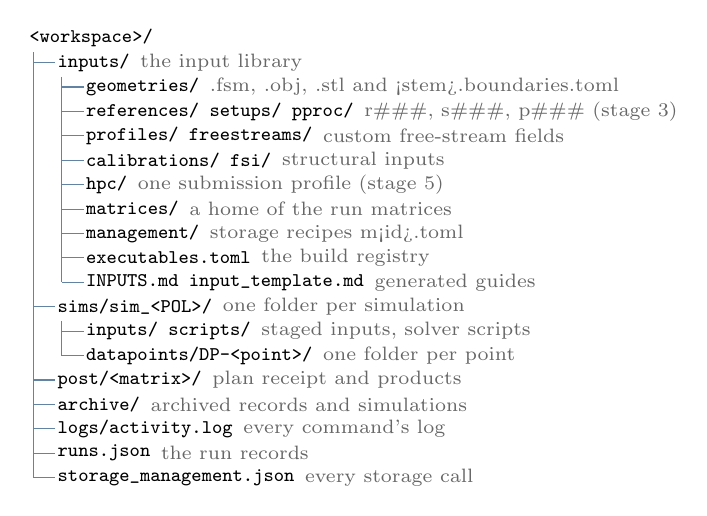
\begin{tikzpicture}
\tn{0}{0}{<workspace>/}{}
\tn{1}{1}{inputs/}{the input library}
\tn{2}{2}{geometries/}{.fsm, .obj, .stl and <stem>.boundaries.toml}
\tn{2}{3}{references/ setups/ pproc/}{r\#\#\#, s\#\#\#, p\#\#\# (stage 3)}
\tn{2}{4}{profiles/ freestreams/}{custom free-stream fields}
\tn{2}{5}{calibrations/ fsi/}{structural inputs}
\tn{2}{6}{hpc/}{one submission profile (stage 5)}
\tn{2}{7}{matrices/}{a home of the run matrices}
\tn{2}{8}{management/}{storage recipes m<id>.toml}
\tn{2}{9}{executables.toml}{the build registry}
\tn{2}{10}{INPUTS.md input_template.md}{generated guides}
\tn{1}{11}{sims/sim_<POL>/}{one folder per simulation}
\tn{2}{12}{inputs/ scripts/}{staged inputs, solver scripts}
\tn{2}{13}{datapoints/DP-<point>/}{one folder per point}
\tn{1}{14}{post/<matrix>/}{plan receipt and products}
\tn{1}{15}{archive/}{archived records and simulations}
\tn{1}{16}{logs/activity.log}{every command's log}
\tn{1}{17}{runs.json}{the run records}
\tn{1}{18}{storage_management.json}{every storage call}
\tv{0}{1}{18}
\tv{1}{2}{10}
\tv{1}{12}{13}
\end{tikzpicture}

\hd{Commands}
\begin{cmdblock}{pyfs-workspace init}{[root]}{Create or complete the tree: every \file{inputs/} folder, \file{sims/}, \file{post/}, \file{archive/}, an \file{inputs/executables.toml} template when none exists, and the generated guides. Safe to run again; the default root is the current folder.}
\end{cmdblock}
\begin{cmdblock}{pyfs-workspace migrate-geometries}{[root]}{Move a flat \file{inputs/geometries/} into one folder per geometry, the layout a new workspace uses.}
\end{cmdblock}
\begin{cmdblock}{pyfs-matrix inventory}{<geometry>}{Write \file{<stem>.boundaries.toml} beside a saved simulation (from its mesh block) or an OBJ (from its groups), and name the solver actions a saved simulation keeps. Needs no executable.}
\opt{--overwrite}{rewrite a saved simulation's sidecar that already exists.}
\opt{--clean}{remove the saved solver actions, keeping \file{<file>.bak-<stamp>} (stage 8).}
\end{cmdblock}
\begin{cmdblock}{pyfs-matrix degenerate}{<geometry>}{Derive the thin blade of a blade mesh (a saved simulation or an OBJ): the sheet midway between its two sides, written beside the source with its boundary inventory. Needs no executable.}
\opt{--root-offset LENGTH}{required: how far the root moves outward along the span, in the mesh's unit.}
\opt{--kind thin-blade}{the one kind, the default.}
\opt{--boundary NAME}{the blade's boundary, for a file that also holds a spinner or a nacelle.}
\opt{--overwrite}{rewrite an existing output.}
\end{cmdblock}

\columnbreak
\hd{Custom free-stream fields}
Each operation writes one file of \file{inputs/freestreams/}, named by \fl{--out STEM} (\texttt{.txt} STRUCTURED, \texttt{.dat} UNSTRUCTURED, the form decides), with its provenance record. Each previews until \fl{--apply}.
\begin{cmdblock}{pyfs-workspace field mirror}{<field>}{Mirror a field through the plane x = 0, y = 0 or z = 0.}
\opt{--plane \{x,y,z\}}{required: the coordinate whose sign changes.}
\opt{--out STEM}{required: the stem of the file written.}
\opt{--workspace DIR}{\fl{--apply} writes (default: preview); \fl{--overwrite} replaces an existing file and its record.}
\end{cmdblock}
\begin{cmdblock}{pyfs-workspace field move}{<field>}{Translate a field so a source point lands on a target point.}
\opt{--source-point X Y Z}{required: the source point (a hub), m, global frame.}
\opt{--target-point X Y Z}{required: where it lands, m, global frame.}
\opt{--out STEM}{\fl{--workspace}, \fl{--apply}, \fl{--overwrite}: as in mirror.}
\end{cmdblock}
\begin{cmdblock}{pyfs-workspace field subtract}{<total> <other>}{Total minus (other minus reference), point by point on one grid.}
\opt{--reference VX VY VZ}{required: the free stream OTHER was solved in, m/s.}
\opt{--tolerance M}{positions closer than this per axis are one point (default 1e-06).}
\opt{--out STEM}{\fl{--workspace}, \fl{--apply}, \fl{--overwrite}: as in mirror.}
\end{cmdblock}
\begin{cmdblock}{pyfs-workspace field time-mean}{<files>}{The time mean of an unsteady run's per-step fields (files or glob patterns).}
\opt{--last K}{average only the last K steps given.}
\opt{--fluctuation}{also write \file{<stem>.fluctuation.csv}, the per-probe standard deviation.}
\opt{--fluctuation-only}{the fluctuation report alone, no field; needs \fl{--last}.}
\opt{--vinf M\_S}{the free-stream speed the fluctuation is also stated against.}
\opt{--tolerance M}{as in subtract.}
\opt{--out STEM}{\fl{--workspace}, \fl{--apply}, \fl{--overwrite}: as in mirror.}
\end{cmdblock}
\begin{cmdblock}{pyfs-workspace field fill-interior}{<field>}{Fill the probes inside the body from the ray outside it.}
\opt{--r-body M}{the body radius about the x axis, m (default 0.38).}
\opt{--out STEM}{\fl{--workspace}, \fl{--apply}, \fl{--overwrite}: as in mirror.}
\end{cmdblock}
\hd{Actuator-disc profiles}
\cmd{pyfs-workspace profile} sections (\fl{--pol}), uni or bp writes \file{inputs/profiles/<STEM>.csv}, a row's \texttt{PROFILE}, scaled to \fl{--thrust} or \fl{--ct}. ELLIPTICAL needs no file.

\columnbreak
\hd{Files}
\rd{inputs/geometries/}{the saved simulation or mesh \cmd{pyfs-matrix inventory} reads.}
\wf{<stem>.boundaries.toml}{beside the geometry: its boundary names, the names every reference alias and pproc family cites.}
\wf{inputs/executables.toml}{the template of the build registry: each build a row may name and its executable.}
\wf{inputs/geometries/README.md}{how to lay out the geometries.}
\wf{inputs/INPUTS.md}{the glossary of every matrix column and input key.}
\wf{inputs/input_template.md}{an example of every input file.}
\wf{inputs/pproc/VARIABLES.md}{with \file{WRITING-EQUATIONS.md}: the pproc variables and how to write an equation.}
\wf{inputs/freestreams/<STEM>}{a custom free-stream field and its provenance record.}

\hd{Common errors}
\err{\cmd{pyfs-workspace init} reports an ambiguous artifact id: two files of \file{geometries/} or \file{profiles/} share one stem (\file{wing.fsm} beside \file{wing.stl}).}{the id is the stem and must be unique: rename or remove the extra file. The tree is still completed.}
\err{The inventory refuses: the sidecar already exists.}{\fl{--overwrite} rewrites a saved simulation's sidecar. An OBJ's sidecar is never rewritten: edit it by hand or remove it.}
\err{A field operation printed what it would write and nothing changed.}{that was the preview: run it again with \fl{--apply}.}
\err{The field file \texttt{<STEM>} already exists.}{choose another \fl{--out}, or replace it and its record with \fl{--overwrite}.}
\err{\fl{--fluctuation-only} refuses.}{it needs \fl{--last} K: the fluctuation of the last K steps.}
\err{A bare stem in a GEOMETRY key is refused.}{name the geometry by its file name, extension included (\file{wing_clean.fsm}).}

\hd{Where to read more}
The pages \textit{The workspace and the workflow}, \textit{The input library and the solver presets} and \textit{Field operations} of the documentation; guide 1, \textit{Workspaces}.
\foot
\end{multicols}

% =====================================================================
\stagepage{2}{The run matrix and its two homes}{The run matrix is the study: one row per polar, each naming its geometry, its three input artifacts, its flight condition and what it sweeps. The row says what is different; the library says what is shared.}
\begin{multicols}{3}
\hd{What it is for}
A matrix is a pipe-delimited text file, \file{<name>.fs}, one row per simulation. \texttt{POL} becomes the simulation id (\file{sims/sim_<POL>/}). \texttt{FLIGHT\_CONDITION} states the flow as \texttt{KEY:value} pairs, and exactly one key carries the word \texttt{sweep}; \texttt{SWEEP\_VALUES} lists its values, so one row is several points. \texttt{-} in a column states nothing.

\hd{The columns, in order}
\begin{tabular}{@{}l@{\ }>{\raggedright\arraybackslash}p{4.9cm}@{}}
\texttt{POL HIDDEN RUN} & id; solver window shown; does the row take part \\
\texttt{AIRCRAFT CONFIGURATION} & what the row is (labels only) \\
\texttt{DESCRIPTION} & your words \\
\texttt{FLIGHT\_CONDITION} & the flow, and what is swept \\
\texttt{SWEEP\_VALUES} & the swept values \\
\texttt{GEOMETRY} & the mesh file, by its file name \\
\texttt{REF SET PPROC} & the coded ids \texttt{r\#\#\#}, \texttt{s\#\#\#}, \texttt{p\#\#\#} \\
\texttt{SYMMETRY SYMMETRY\_LOADS} & what was meshed, which loads come back \\
\texttt{NCPUS WALLTIME} & processors; wall clock with its unit (\texttt{4h}) \\
\texttt{FS\_BUILD} & the build the row wants, e.g. \texttt{\fsbuild} \\
\texttt{WORKFLOW} & the run type: \texttt{steady}, \texttt{unsteady}, \texttt{unsteady\_rotor}, \texttt{qsteady\_rotor}, or \texttt{LEGACY} (a recipe) \\
\texttt{VAR\_NAMES\_VALUES} & every other key, \texttt{KEY: value} pairs separated by \texttt{/} \\
\end{tabular}

\hd{Reading one row}
\begin{tabular}{@{}l@{\ \ }l@{}}
\texttt{POL} & \texttt{7002}: the simulation \file{sims/sim_7002/} \\
\texttt{FLIGHT\_CONDITION} & \texttt{TASmps:30.0, REmi:1.20, ALPHA:sweep} \\
\texttt{SWEEP\_VALUES} & \texttt{0.0,2.0}: two angles, two points \\
\texttt{GEOMETRY} & \texttt{wing.fsm}, staged in \file{inputs/geometries/} \\
\texttt{REF SET PPROC} & \texttt{r003 s002 p001} \\
\texttt{FS\_BUILD WORKFLOW} & \texttt{26.120 steady} \\
\texttt{VAR\_NAMES\_VALUES} & \texttt{VELOCITY: 30.0} \\
\end{tabular}

\hd{Several matrices in one workspace}
Each matrix keeps its own \file{post/<matrix>/} folder, named after its file stem, with its own plan receipt and sweep table. A POL may be used by one row of one matrix only: \cmd{pyfs-matrix plan} finds a repeat, and its option to renumber is on stage 4.

\hd{How a point is named}
The point name writes each flight-condition variable as a code and a fixed-width integer: \texttt{M144RE438AL+000BE+000J+080}. Scripts and exports are \texttt{P<sim>-<name>}, the run id is \texttt{<campaign>/sim\_<POL>/<name>}, and a steady row is one job, \texttt{<campaign>/sim\_<POL>/sweep}.

\columnbreak
\hd{Figure: the two homes and the one lookup}
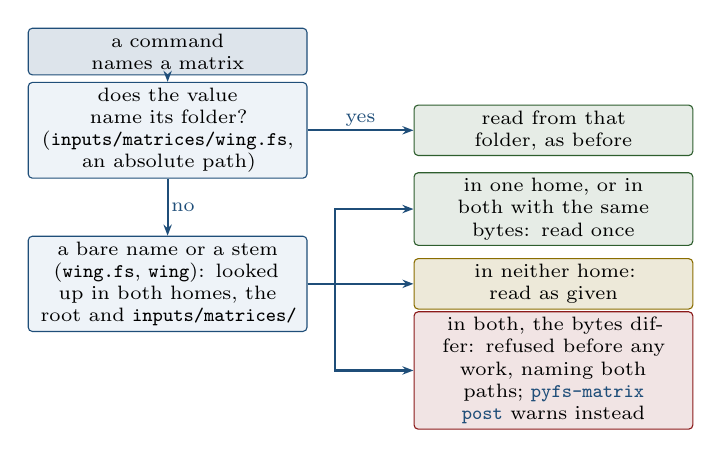
\begin{tikzpicture}
\node[box,text width=3.4cm,fill=acc!15] (q) at (0,0) {a command names a matrix};
\node[box,text width=3.4cm] (d) at (0,-1.0) {does the value name its folder? (\pth{inputs/matrices/wing.fs}, an absolute path)};
\node[box,text width=3.4cm,fill=ok!12,draw=ok] (r1) at (4.9,-1.0) {read from that folder, as before};
\node[box,text width=3.4cm] (l) at (0,-2.95) {a bare name or a stem (\pth{wing.fs}, \pth{wing}): looked up in both homes, the root and \pth{inputs/matrices/}};
\node[box,text width=3.4cm,fill=ok!12,draw=ok] (o1) at (4.9,-2.0) {in one home, or in both with the same bytes: read once};
\node[box,text width=3.4cm,fill=wait!15,draw=wait] (o2) at (4.9,-2.95) {in neither home: read as given};
\node[box,text width=3.4cm,fill=bad!12,draw=bad] (o3) at (4.9,-4.05) {in both, the bytes differ: refused before any work, naming both paths; \cmd{pyfs-matrix post} warns instead};
\draw[arr] (q) -- (d);
\draw[arr] (d) -- node[note,above]{yes} (r1);
\draw[arr] (d) -- node[note,right]{no} (l);
\draw[arr] (l.east) -- ++(0.35,0) |- (o1.west);
\draw[arr] (l.east) -- ++(0.35,0) |- (o2.west);
\draw[arr] (l.east) -- ++(0.35,0) |- (o3.west);
\end{tikzpicture}

\vspace{2pt}
Every command that takes a matrix reads it through this lookup: \cmd{pyfs-matrix upgrade}, \cmd{pyfs-matrix convert}, \cmd{pyfs-matrix plan}, \cmd{pyfs-matrix inspect-setups}, \cmd{pyfs-matrix run}, \cmd{pyfs-matrix post}, \cmd{pyfs-matrix rebuild} and \cmd{pyfs-matrix rename}. \cmd{pyfs-matrix upgrade} and \cmd{pyfs-matrix convert} take no workspace and look in the current folder.

\hd{Commands}
\begin{cmdblock}{pyfs-matrix upgrade}{<matrix>}{Convert a matrix written under an older layout to the current one.}
\opt{--in-place}{rewrite the file (default: print to standard output).}
\opt{--inputs DIR}{also move \file{inputs/groups/e001.toml} to \file{inputs/pproc/p001.toml} under \texttt{[groups]}; needs \fl{--in-place}.}
\end{cmdblock}
\begin{cmdblock}{pyfs-matrix convert}{<matrix>}{Emit the native \file{campaign.toml} equivalent of a matrix.}
\opt{--fs-exe PATH}{required: the executable, never guessed.}
\opt{--name NAME}{the campaign name; required here, as there is no workspace.}
\opt{--fs-version V}{the build for rows whose FS\_BUILD cell is empty.}
\opt{--recipe CODE=MODULE:FUNCTION}{a LEGACY recipe code (repeatable).}
\opt{-o, --output FILE}{write here instead of standard output.}
\end{cmdblock}
\begin{cmdblock}{pyfs-matrix rename}{}{Rename a workspace written under 0.20.x to the point names of 0.21.0 (folders, scripts, records, plan).}
\opt{--workspace DIR}{the campaign root (default: current folder).}
\opt{--dry-run}{print what would move and change nothing; read it first.}
\end{cmdblock}

\columnbreak
\hd{The optional workbook (the excel extra)}
Save and close the workbook first. A read imports matrices into its Runs sheet, a write exports Runs to matrices; both go through a preview, then an apply.
\begin{cmdblock}{python -m pyflightstream.workspace.excel create}{<output>}{Create a new macro-free workbook.}
\opt{--workspace DIR}{required: the campaign it belongs to.}
\end{cmdblock}
\begin{cmdblock}{python -m pyflightstream.workspace.excel preview}{<workbook>}{Write a batch, its JSON and an HTML beside it; change nothing.}
\opt{--workspace DIR}{required.}
\opt{--direction \{read,write\}}{required: read imports, write exports.}
\opt{--batch FILE}{required: the pending transaction; keep it unchanged.}
\opt{--matrix FILE}{select a subset (repeatable).}
\end{cmdblock}
\begin{cmdblock}{python -m pyflightstream.workspace.excel apply}{<batch>}{Apply one fresh reviewed batch; each batch is single use.}
\end{cmdblock}
\begin{cmdblock}{python -m pyflightstream.workspace.excel cancel}{<batch>}{Cancel a preview; nothing changes.}
\end{cmdblock}
\begin{cmdblock}{python -m pyflightstream.workspace.excel check}{<workbook>}{Validate its Runs and Dictionary.}
\end{cmdblock}

\hd{Files}
\rd{<name>.fs}{in the workspace root or in \file{inputs/matrices/}, the two homes.}
\wf{campaign.toml}{written by \cmd{pyfs-matrix convert}.}
\rd{inputs/sync-workspaces.toml}{names the workspace that owns each matrix (stage 6).}

\hd{Common errors}
\err{One stem in both homes with different bytes: every command refuses, naming both paths.}{keep one copy, or make the two identical.}
\err{The plan warns that the matrix lies outside the workspace's matrix folders.}{move it to the root or \file{inputs/matrices/}: \cmd{pyfs-matrix sync} and the repeated-POL check see only those two.}
\err{A WALLTIME cell is a bare number.}{write its unit: \texttt{240m}, \texttt{4h}, \texttt{90s}, \texttt{1d}.}
\err{A fact is stated in its column and as a key of \texttt{VAR\_NAMES\_VALUES}.}{refused naming both: keep one home for it.}
\err{A row moved off LEGACY keeps an \texttt{FSM\_FILE} key.}{refused at plan naming the key: rename it to \texttt{GEOMETRY}.}
\err{\fl{--inputs} without \fl{--in-place}.}{the matrix cells that name the files are rewritten with them: add \fl{--in-place}.}
\foot
\end{multicols}

% =====================================================================
\stagepage{3}{The reference, setup and pproc artifacts}{Three small files a row cites by coded id: the reference \texttt{r\#\#\#} (what the numbers are measured against and what the parts are called), the setup \texttt{s\#\#\#} (how the solver runs) and the pproc \texttt{p\#\#\#} (what is written down afterwards).}
\begin{multicols}{3}
\hd{What it is for}
A study is many runs that share almost everything. What they share lives in these files, split by how often it changes, and a row names one of each: \texttt{REF}, \texttt{SET} and \texttt{PPROC}. The letter of a coded id declares its kind, so a mistyped number cannot reach another kind's file.

\hd{Figure: what a row resolves to}
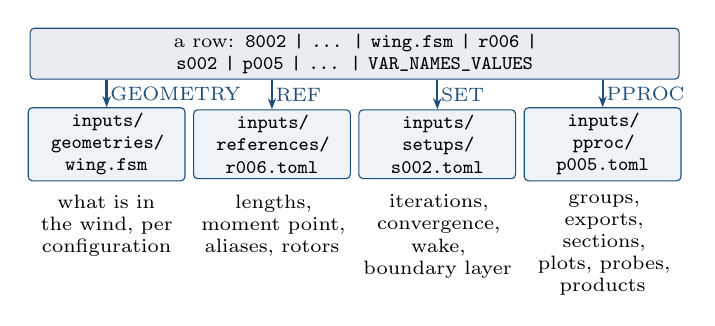
\begin{tikzpicture}
\node[box,text width=8.1cm,fill=acc!10] (row) at (3.15,0) {a row: \pth{8002 | ... | wing.fsm | r006 | s002 | p005 | ... | VAR_NAMES_VALUES}};
\node[box,text width=1.85cm] (g) at (0,-1.15) {\pth{inputs/}\\\pth{geometries/}\\\pth{wing.fsm}};
\node[box,text width=1.85cm] (r) at (2.1,-1.15) {\pth{inputs/}\\\pth{references/}\\\pth{r006.toml}};
\node[box,text width=1.85cm] (s) at (4.2,-1.15) {\pth{inputs/}\\\pth{setups/}\\\pth{s002.toml}};
\node[box,text width=1.85cm] (p) at (6.3,-1.15) {\pth{inputs/}\\\pth{pproc/}\\\pth{p005.toml}};
\foreach \n/\c in {g/GEOMETRY,r/REF,s/SET,p/PPROC}{\draw[arr] (\n.north |- row.south) -- node[note,right,font=\fontsize{6.6}{7.6}\selectfont]{\c} (\n.north);}
\node[note,text width=1.9cm,anchor=north,align=center] at (0,-1.75) {what is in the wind, per configuration};
\node[note,text width=1.9cm,anchor=north,align=center] at (2.1,-1.75) {lengths, moment point, aliases, rotors};
\node[note,text width=1.9cm,anchor=north,align=center] at (4.2,-1.75) {iterations, convergence, wake, boundary layer};
\node[note,text width=1.9cm,anchor=north,align=center] at (6.3,-1.75) {groups, exports, sections, plots, probes, products};
\end{tikzpicture}

\hd{The reference \textmd{\texttt{r\#\#\#}}}
\texttt{area\_m2}, \texttt{chord\_m}, \texttt{span\_m} and \texttt{[moment\_point]} are what every coefficient is divided by and taken about. \texttt{[aliases]} names sets of boundaries once (\texttt{airframe = ["Body", "Base"]}); a member the opened mesh lacks is left out, so one reference serves several geometries. A block with \texttt{kind = "rotor"} is a rotor: hub, \texttt{axis}, \texttt{rpm\_sign}, \texttt{diameter\_m}, its blade families; a row then names the rotor and nothing else about it.

\hd{A rotor block of the reference}
{\ttfamily\scriptsize\obeylines\obeyspaces%
[PORT]
kind = "rotor"
x\_m = 4.5\ \ \ \ \ \ \ \ \ \ \ \ \# the hub; y\_m, z\_m likewise
axis = "X"\ \ \ \ \ \ \ \ \ \ \# what it turns about
rpm\_sign = 1\ \ \ \ \ \ \ \ \# which way
diameter\_m = 3.6576\ \# what J resolves against
families\_blades = ["Blade1"]\ \# the count is its length
}
\hd{Starting a library}
Copy a working \file{inputs/} whole, delete the artifacts you do not need, edit the reference to your own lengths and boundary names, then write one matrix row and plan it.

\columnbreak
\hd{The setup \textmd{\texttt{s\#\#\#}}}
The knobs set once for a study: iterations, convergence, the wake, the boundary-layer type, \texttt{solver\_model}, \texttt{moments\_model} (\texttt{PRESSURE} or \texttt{VORTICITY}). The time step is not here: it is what a point is, so it lives on the row. A row may state setup keys over its preset in \texttt{VAR\_NAMES\_VALUES}, under their native names, for that row only: the plan warns, a key the preset does not state or states equally is accepted, and the run record lists them under \texttt{from\_row}.

\hd{The pproc \textmd{\texttt{p\#\#\#}}}
Boundary groups, exports, sectional distributions, force plots, probe lines, sampled fields and the product tables. The frame decides how an entry expands:

\begin{tabular}{@{}l@{\ \ }l@{}}
\texttt{frame =} & you get \\\hline
\texttt{MRP}, or a declared frame & one, over the whole cited set \\
\texttt{SMRP} or \texttt{RMRP} & one per rotor, in its own frame \\
\texttt{LOCAL\_AXIS} & one per blade, in its frame \\
\end{tabular}

A second artifact can be extracted after the run, with no solve: \texttt{ADDITIONAL\_PPROC: p<id>} on the row and \cmd{pyfs-matrix post} with its additional post (stage 7).

\hd{Commands}
These options of \cmd{pyfs-matrix plan} concern the artifacts; the rest of the plan is stage 4.
\begin{cmdblock}{pyfs-matrix plan}{<matrix>}{Bind the matrix to the library and pre-flight every point.}
\opt{--setup-guidelines}{write \file{inputs/setups/SETUP_GUIDELINES.md}, keeping your edits.}
\opt{--setup-standards}{write the commented s9XX setup standards, keeping your edits.}
\opt{--ignore-missing-families [true|false]}{true (default): a family the opened mesh lacks is left out; false refuses the point.}
\opt{--no-ignore-missing-families}{the same as \texttt{false}, as a flag.}
\end{cmdblock}

\columnbreak
\hd{Files}
\rd{inputs/references/r006.toml}{the reference a row's REF cell names.}
\rd{inputs/setups/s002.toml}{the setup preset of the SET cell.}
\rd{inputs/pproc/p005.toml}{the post-processing artifact of the PPROC cell.}
\rd{<stem>.boundaries.toml}{the boundary names aliases and families must match.}
\wf{inputs/setups/SETUP_GUIDELINES.md}{the setup guidance, on request.}
\wf{inputs/pproc/VARIABLES.md}{rewritten when a pproc gains a glossary.}

\hd{Common errors}
\err{A row states a setup key the preset states with another value.}{refused at plan, naming both values: change the row or the preset.}
\err{A rotor row's setup states \texttt{vorticity\_drag\_families} and \texttt{moments\_model = PRESSURE}.}{refused at plan: state \texttt{VORTICITY} or drop the drag list. Unstated, a rotor row with the list takes \texttt{VORTICITY} and the plan warns.}
\err{The plan warns that a section or plot group names a family a row's geometry lacks.}{a misspelled family is named the same way: check the name against \file{<stem>.boundaries.toml}. The point plans; \fl{--ignore-missing-families} \texttt{false} refuses it instead.}
\err{Both \fl{--ignore-missing-families} and \fl{--no-ignore-missing-families} are stated.}{refused: state one.}
\err{A coefficient looks off by a constant factor.}{check \texttt{area\_m2}, \texttt{chord\_m} and \texttt{span\_m} of the cited reference: every coefficient is divided by them.}
\err{An unsteady row states no averaging window.}{every unsteady row must state one: \texttt{LAST\_REVS\_AVG} in revolutions, or \texttt{LAST\_ITERS\_AVG} in time iterations.}

\hd{Where to read more}
Guide 3, \textit{References}; guide 4, \textit{Solver setup}; guide 5, \textit{Post-processing definitions}; the documentation pages \textit{The reference artifact} and \textit{The post-processing artifact and its products}.
\foot
\end{multicols}

% =====================================================================
\stagepage{4}{Plan: the pre-flight}{The plan binds every row to the library, builds every script in a dry run and says READY or BLOCKED with the reason, spending no solver time. It is mandatory: it writes the receipt a run asks for.}
\begin{multicols}{3}
\hd{What it is for}
Always plan before you run: a blocked point costs a message, a bad run costs the license. The plan prints its answer in blocks, writes \file{post/<matrix>/plan.json} pinned to the digest of the matrix it read, and a run refuses a matrix edited since. Its warnings refuse nothing; read them before you run. Exit code 1 when a point is blocked, 0 otherwise.

\hd{Figure: the plan and its receipt}
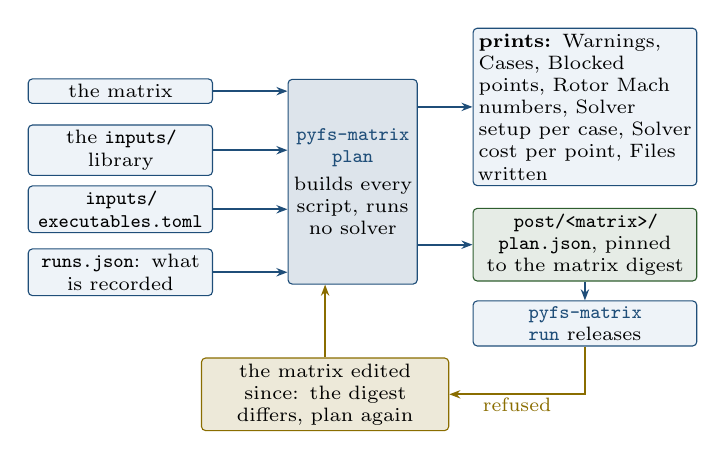
\begin{tikzpicture}
\node[box,text width=2.2cm] (m) at (0,0) {the matrix};
\node[box,text width=2.2cm] (i) at (0,-0.75) {the \pth{inputs/} library};
\node[box,text width=2.2cm] (x) at (0,-1.5) {\pth{inputs/}\\\pth{executables.toml}};
\node[box,text width=2.2cm] (rj) at (0,-2.3) {\pth{runs.json}: what is recorded};
\node[box,text width=1.5cm,minimum height=2.6cm,fill=acc!15] (p) at (2.95,-1.15) {\cmd{pyfs-matrix plan}\\[2pt]builds every script, runs no solver};
\node[box,text width=2.7cm,align=left] (b) at (5.9,-0.2) {\textbf{prints:} Warnings, Cases, Blocked points, Rotor Mach numbers, Solver setup per case, Solver cost per point, Files written};
\node[box,text width=2.7cm,fill=ok!12,draw=ok] (pj) at (5.9,-1.95) {\pth{post/<matrix>/}\\\pth{plan.json}, pinned to the matrix digest};
\node[box,text width=2.7cm] (run) at (5.9,-2.95) {\cmd{pyfs-matrix run} releases};
\node[box,text width=3.0cm,fill=wait!15,draw=wait] (e) at (2.6,-3.85) {the matrix edited since: the digest differs, plan again};
\foreach \n in {m,i,x,rj}{\draw[arr] (\n.east) -- (\n.east -| p.west);}
\draw[arr] (p.east |- b.west) -- (b.west);
\draw[arr] (p.east |- pj.west) -- (pj.west);
\draw[arr] (pj) -- (run);
\draw[arr,wait] (run.south) |- node[note,below,pos=0.75]{refused} (e.east);
\draw[arr,wait] (e.north) -- (e.north |- p.south);
\end{tikzpicture}

\hd{A typical sequence}
{\ttfamily\scriptsize pyfs-matrix plan study.fs --workspace . --fs-version 26.123\\
pyfs-matrix plan study.fs --workspace . --cost\\
pyfs-matrix run\ \ study.fs --workspace . --fs-version 26.123\par}
The first plan names what blocks; fix it and plan again until every point is READY. The second adds the cost table. The run gives the plan's values again.

\hd{The output blocks}
\textbf{Warnings} go to standard error; everything else to standard output. \textbf{Cases} counts the points ready, blocked and already recorded. \textbf{Blocked points} names each one and why. \textbf{Rotor Mach numbers}: tip and helical Mach per rotor and point. \textbf{Solver setup per case}: model, boundary layer, viscous coupling, aliases. \textbf{Files written}: the receipt and any guide. \file{logs/activity.log} keeps every line.

\columnbreak
\hd{Commands}
\begin{cmdblock}{pyfs-matrix plan}{<matrix>}{Pre-flight every point; no solver runs. Its alias is \cmd{pyfs-matrix inspect-setups}. The artifact options are on stage 3.}
\opt{--workspace DIR}{the campaign root with \file{inputs/} (default: current folder).}
\opt{--name NAME}{the campaign name (default: the workspace folder's name).}
\opt{--fs-version V}{the build for rows whose FS\_BUILD cell is empty, e.g. \texttt{\fsbuild}.}
\opt{--fs-exe PATH}{an executable override; mandatory for a row whose FS\_BUILD says MANUAL, otherwise the build resolves through \file{inputs/executables.toml}.}
\opt{--workflow CODE=NAME}{a legacy script code to a run type (repeatable), the mapping \cmd{pyfs-matrix run} takes.}
\opt{--sims SIM [SIM ...]}{plan only these simulations, space separated (\texttt{2031 2032}); the matrix is not edited.}
\opt{--points POINT [POINT ...]}{with \fl{--sims}: only these points, by the point name the plan prints.}
\opt{--recipe CODE=MODULE:FUNCTION}{a LEGACY row's recipe (repeatable).}
\opt{--point-name TPL}{the naming template; default \texttt{\{polar\}}, which is \texttt{P<sim>-<point name>}; also \texttt{\{point\}} \texttt{\{alpha\}} \texttt{\{beta\}} \texttt{\{mach\}} \texttt{\{advance\_ratio\}} \texttt{\{sim\}} \texttt{\{campaign\}}.}
\opt{--cost}{table each point's expected cost: mesh size, marked trailing edges, farfield layers, viscous coupling, steady or unsteady, time iterations, processors, and an EXPECTED wall time fitted on this workspace's own runs (\texttt{unknown} without a comparable run).}
\opt{--inflow-fft}{for each \texttt{qsteady\_rotor} wheel point in a custom inflow: the harmonics one blade meets, \texttt{k\_eff}, \texttt{n\_max} and the suggested \texttt{PASSAGE\_POSITIONS}; warns when the row states fewer.}
\opt{--update-ids}{(also \fl{--updateIDs}) REWRITE this matrix so no POL repeats one used elsewhere in the workspace; written before the plan runs, and kept if the plan then refuses.}
\opt{--accept-unregistered-build}{allow an installed build other than the registered one; its compatibility is your responsibility and every record says so.}
\opt{--verbose}{every warning in full, and the started and finished lines of each continuation.}
\end{cmdblock}

\hd{Reading the cost table}
The expected wall time is an extrapolation from this workspace's recorded runs, and the table carries the number of samples behind it. A new workspace reads \texttt{unknown}: run a few points first, then plan again with \fl{--cost}.

\columnbreak
\hd{Files}
\rd{<matrix>.fs}{from either home (stage 2).}
\rd{inputs/}{every artifact a row names, and \file{inputs/executables.toml} for each FS\_BUILD.}
\rd{runs.json}{which points are already recorded.}
\wf{post/<matrix>/plan.json}{the receipt \cmd{pyfs-matrix run} asks for, pinned to the matrix digest.}
\wf{logs/activity.log}{every line the plan printed, and the detail \fl{--verbose} adds.}
\wf{<matrix>.fs}{rewritten only by \fl{--update-ids}, each change printed.}

\hd{Common errors}
\err{A point is BLOCKED, with the reason under \textit{Blocked points}.}{fix the row or the input it names, then plan again; a blocked point never runs.}
\err{The build installed is not the one registered for the row's version.}{refused: install the registered build, or pass \fl{--accept-unregistered-build}, recorded in \file{plan.json} and on every record.}
\err{A row's FS\_BUILD cell is empty and no fallback is given.}{fill the cell, or pass \fl{--fs-version}.}
\err{A run type refuses the build: outside the range it covers.}{the refusal names the builds it covers and the commands that decided it: choose one of them in FS\_BUILD.}
\err{A POL repeats one stated in another matrix or earlier in this file.}{\fl{--update-ids} renumbers the repeated rows; a row whose POL already has runs of this matrix is refused rather than moved.}
\err{The plan warns: helical Mach of 1 or more on some points.}{a warning, not a refusal: check the rotor speed of those points.}
\err{The plan lists points a \texttt{RESTART} key does not continue.}{\texttt{FINISH\_PENDING} on a CONVERGED run is refused with the reason; use \texttt{ADDITIONAL\_REVS} or \texttt{ADDITIONAL\_ITERS}.}
\err{The plan warns that an unsteady row's geometry carries saved solver actions.}{clean it with \cmd{pyfs-matrix inventory} \fl{--clean} (stage 8); the plan never refuses on that account.}

\hd{Where to read more}
The documentation page \textit{Planning a campaign and what it costs}.
\foot
\end{multicols}

% =====================================================================
\stagepage{5}{Run: on this machine or on the cluster}{The run builds every active point's script and executes it: on Windows locally, on Linux with a submission profile by submitting each point to the scheduler. Every point lands in the records with exactly one status.}
\begin{multicols}{3}
\hd{What it is for}
A run needs a current plan. Each point runs in its own datapoint folder, \file{sims/sim_<POL>/datapoints/DP-<point>/}, where its outputs are filed; a steady row is one job over all its points, run in the simulation folder. A local point is recorded when it ends; a submitted point is recorded \texttt{SUBMITTED} and finished by \cmd{pyfs-matrix collect} (stage 6). There is no separate submit command.

\hd{Figure: where a point runs}
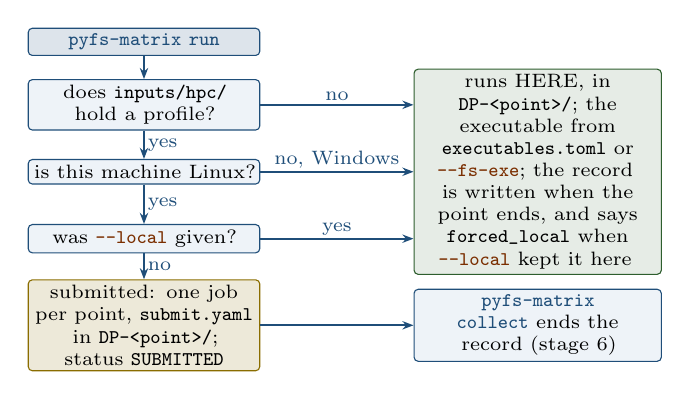
\begin{tikzpicture}
\node[box,text width=2.8cm,fill=acc!15] (r) at (0,0) {\cmd{pyfs-matrix run}};
\node[box,text width=2.8cm] (h) at (0,-0.8) {does \pth{inputs/hpc/} hold a profile?};
\node[box,text width=2.8cm] (l) at (0,-1.65) {is this machine Linux?};
\node[box,text width=2.8cm] (f) at (0,-2.5) {was \fl{--local} given?};
\node[box,text width=3.0cm,minimum height=2.3cm,fill=ok!12,draw=ok] (loc) at (5.0,-1.65) {runs HERE, in \pth{DP-<point>/}; the executable from \pth{executables.toml} or \fl{--fs-exe}; the record is written when the point ends, and says \pth{forced_local} when \fl{--local} kept it here};
\node[box,text width=2.8cm,fill=wait!15,draw=wait] (sub) at (0,-3.6) {submitted: one job per point, \pth{submit.yaml} in \pth{DP-<point>/}; status \pth{SUBMITTED}};
\node[box,text width=3.0cm] (col) at (5.0,-3.6) {\cmd{pyfs-matrix collect} ends the record (stage 6)};
\draw[arr] (r) -- (h);
\draw[arr] (h) -- node[note,right]{yes} (l);
\draw[arr] (l) -- node[note,right]{yes} (f);
\draw[arr] (f) -- node[note,right]{no} (sub);
\draw[arr] (h.east) -- node[note,above]{no} (h.east -| loc.west);
\draw[arr] (l.east) -- node[note,above]{no, Windows} (l.east -| loc.west);
\draw[arr] (f.east) -- node[note,above]{yes} (f.east -| loc.west);
\draw[arr] (sub) -- (col);
\end{tikzpicture}

\hd{A session on the cluster}
{\ttfamily\scriptsize pyfs-matrix plan study.fs --workspace .\\
pyfs-matrix run\ \ study.fs --workspace .\\
pyfs-matrix collect --workspace . --watch\par}
On Linux with a profile the run submits every point and returns; collect then sweeps until nothing is outstanding. On Windows the same run executes the points here and needs no collect.

\hd{The submission profile}
One \file{inputs/hpc/h001.toml} per workspace (two are refused): the descriptor and its fields, the submit command, \texttt{[builds]} (the scheduler's name of each build, e.g. \texttt{"26.123" = "26.1"}) and \texttt{[log]} (\texttt{export\_log}, \texttt{native\_log}, \texttt{job\_end\_files}).

\columnbreak
\hd{Commands}
\begin{cmdblock}{pyfs-matrix run}{<matrix>}{Run every active point and write the sweep table.}
\opt{--resume}{skip points already recorded, so a grown matrix runs only its new points; without it a recorded point refuses.}
\opt{--force-rerun POINT}{REDO a recorded point, by point name, full run id or a steady row's job id (repeatable): the records and outputs are archived first, nothing is deleted.}
\opt{--force-rerun-all}{REDO every recorded point; the count of points and jobs, the licenses it spends, prints first.}
\opt{--sims SIM [SIM ...]}{run only these simulations, space separated (\texttt{2031 2032}); with \fl{--force-rerun-all}, redo only these.}
\opt{--points POINT [POINT ...]}{with \fl{--sims}: run only these points, by the point name the plan prints; refused beside \fl{--force-rerun-all}.}
\opt{--local}{run on THIS machine instead of submitting: a Linux workstation, or a smoke test.}
\opt{--progress-every N}{a local unsteady point reports every N steps (default 10; 0 is silent).}
\opt{--sweep-csv FILE}{the sweep table (default \file{post/<matrix>/campaign_sweep.csv}).}
\opt{--workflow CODE=NAME}{a legacy script code to a run type: \texttt{steady}, \texttt{unsteady}, \texttt{unsteady\_rotor}, \texttt{qsteady\_rotor} (repeatable).}
\opt{--workspace DIR}{\fl{--name NAME}, \fl{--fs-version V}, \fl{--fs-exe PATH}, \fl{--recipe CODE=MODULE:FUNCTION}, \fl{--point-name TPL}: as in plan; give the plan's values.}
\opt{--ignore-missing-families [true|false]}{and \fl{--no-ignore-missing-families}: as in plan.}
\opt{--accept-unregistered-build}{as in plan; every record says it was used and carries the build the solver printed.}
\opt{--pproc-warnings}{print the post-processing warnings, grouped.}
\opt{--verbose}{every warning in full, one line per repeated item.}
\end{cmdblock}

\hd{Redoing a point}
A correction that does not change a point's name (a pproc, a geometry, a solver variable, a wall clock) keeps its identity: plan again, then \fl{--force-rerun} it. A correction to \texttt{FLIGHT\_CONDITION} changes the name: it is a new point, and \fl{--resume} runs it beside the old record.

\columnbreak
\hd{Files}
\rd{post/<matrix>/plan.json}{must be current: the digest of the matrix it read.}
\rd{inputs/executables.toml}{each FS\_BUILD to its executable.}
\rd{inputs/hpc/h001.toml}{the submission profile, when the workspace has one.}
\wf{sims/sim_<POL>/scripts/}{the generated solver scripts, \file{P<sim>-<point>.txt}.}
\wf{sims/sim_<POL>/datapoints/DP-<point>/}{the point's outputs, its descriptor when submitted, its wall-clock state.}
\wf{runs.json}{one record per point or steady job; \file{runs.json.lock} while it is written.}
\wf{post/<matrix>/campaign_sweep.csv}{the sweep table of this matrix.}
\wf{archive/runs-<stamp>.json}{the manifest before a forced re-run; each redone point's outputs go to its own \file{archive/<stamp>/}.}

\hd{Common errors}
\err{\textit{no plan for this matrix, and since v0.17.0 a run needs one}.}{run \cmd{pyfs-matrix plan} with the same matrix first.}
\err{The matrix was edited after the plan.}{refused until planned again: the receipt is pinned to the matrix digest.}
\err{A point is already recorded and refuses.}{the refusal counts the points recorded and those \fl{--resume} would run, and prints the command that continues; \fl{--force-rerun} redoes a point. \fl{--resume} and \fl{--force-rerun} together are refused.}
\err{\fl{--sims} names an id, or \fl{--points} a point, the matrix does not carry; or \fl{--points} comes without \fl{--sims}.}{refused before anything runs, naming the ids or points that exist.}
\err{\fl{--force-rerun} names a point no record carries.}{refused: copy the name or run id the refusal printed.}
\err{\fl{--force-rerun-all} is refused.}{beside \fl{--resume}, \fl{--force-rerun} or \fl{--points}, for a \fl{--sims} id the matrix does not carry, or when nothing of the selection is recorded.}
\err{Two profiles in \file{inputs/hpc/}.}{refused rather than guessed: keep the one of this cluster.}
\err{The profile has no \texttt{[builds]} line for a row's build.}{refused before any point is submitted: add the line.}
\err{A WALLTIME cell written as a bare number is refused by name.}{write it with its unit (stage 2).}
\err{\fl{--resume} on a simulation a rebuild refused (stage 8).}{never: without a record the resume runs it again. Settle the rebuild first.}
\foot
\end{multicols}

% =====================================================================
\stagepage{6}{Collect and the run records}{A submitted point comes back when its outputs land: collect waits for them, files them, judges the run and updates its record. The records, \texttt{runs.json}, are the study's evidence; sync keeps a workstation and a cluster in agreement.}
\begin{multicols}{3}
\hd{What it is for}
For every \texttt{SUBMITTED} record, \cmd{pyfs-matrix collect} waits until the declared outputs are present and SETTLED (the same size and time at two observations), collects them, assesses the run, writes its terminal status, then posts (stage 7). A local run needs no collect. Every executed point lands in exactly one status: a silently skipped point is impossible.

\hd{Figure: the life of a run record}
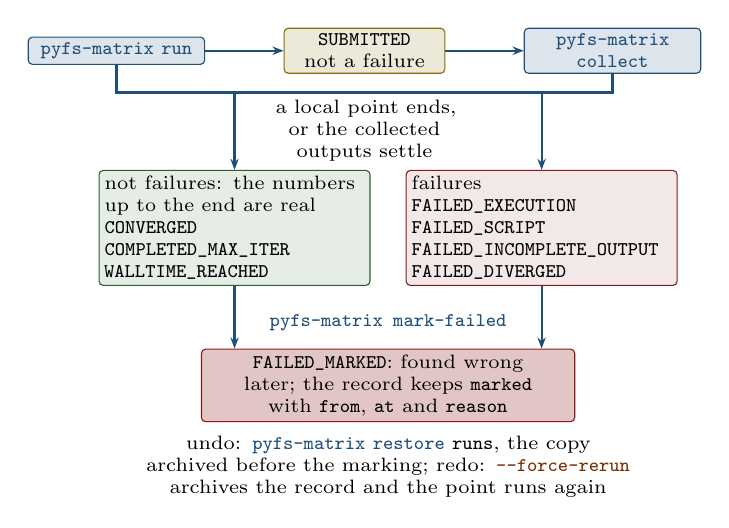
\begin{tikzpicture}
\node[box,text width=2.1cm,fill=acc!15] (run) at (0,0) {\cmd{pyfs-matrix run}};
\node[box,text width=1.9cm,fill=wait!15,draw=wait] (sub) at (3.15,0) {\pth{SUBMITTED}\\not a failure};
\node[box,text width=2.1cm,fill=acc!15] (col) at (6.3,0) {\cmd{pyfs-matrix collect}};
\draw[arr] (run) -- (sub);
\draw[arr] (sub) -- (col);
\draw[thick,acc] (run.south) -- ++(0,-0.35) coordinate (a) -- (a -| col.south) coordinate (c) -- (col.south);
\node[note,text width=2.7cm,align=center,anchor=north] at ($(a)!0.5!(c)+(0,-0.05)$) {a local point ends, or the collected outputs settle};
\node[box,text width=3.3cm,fill=ok!12,draw=ok,align=left] (good) at (1.5,-2.25) {not failures: the numbers up to the end are real\\\pth{CONVERGED}\\\pth{COMPLETED_MAX_ITER}\\\pth{WALLTIME_REACHED}};
\node[box,text width=3.3cm,fill=bad!10,draw=bad,align=left] (bad) at (5.4,-2.25) {failures\\\pth{FAILED_EXECUTION}\\\pth{FAILED_SCRIPT}\\\pth{FAILED_INCOMPLETE_OUTPUT}\\\pth{FAILED_DIVERGED}};
\draw[arr] (good.north |- a) -- (good.north);
\draw[arr] (bad.north |- a) -- (bad.north);
\node[box,text width=4.6cm,fill=bad!25,draw=bad] (mk) at (3.45,-4.25) {\pth{FAILED_MARKED}: found wrong later; the record keeps \pth{marked} with \pth{from}, \pth{at} and \pth{reason}};
\draw[arr] (good.south) -- (good.south |- mk.north);
\node[note,align=center] at (3.45,-3.45) {\cmd{pyfs-matrix mark-failed}};
\draw[arr] (bad.south) -- (bad.south |- mk.north);
\node[note,text width=7.6cm,align=center,anchor=north] at (3.45,-4.85) {undo: \cmd{pyfs-matrix restore} \pth{runs}, the copy archived before the marking; redo: \fl{--force-rerun} archives the record and the point runs again};
\end{tikzpicture}

\vspace{1pt}
\hd{What a record carries}
Which run it was (\texttt{run\_id}, \texttt{point\_name}, \texttt{sweep\_name}), which build ran it, the hashes of the script and the inputs, how the solver was called (\texttt{executor}), where it ran (\texttt{working\_dir}), how it ended (\texttt{status}), how long it took and which files it produced. Nothing is inferred from a folder name afterwards.

\texttt{COMPLETED\_MAX\_ITER} and \texttt{WALLTIME\_REACHED} are not failures: the numbers up to the cap are real. Every reader that asks whether a status begins with \texttt{FAILED} treats \texttt{FAILED\_MARKED} as a failure. A forced re-run archives the record and the point runs again.

\columnbreak
\hd{Commands}
\begin{cmdblock}{pyfs-matrix collect}{}{Collect the outputs of every SUBMITTED record when they land, then post.}
\opt{--watch}{keep sweeping until nothing is outstanding (default: one sweep).}
\opt{--discard-walltime}{mark clock-stopped points failed before post; keep outputs. Grouped plans rerun them from the start; default-mode plans need an explicit rerun.}
\opt{--watch-interval S}{seconds between sweeps under watch (default 60).}
\opt{--interval S}{seconds between the two observations that decide settled (default 2).}
\opt{--rounds N}{stop a watch after N sweeps.}
\opt{--sims IDS}{only the SUBMITTED records of these simulations (\texttt{2006,2007}), and their post.}
\opt{--no-post}{collect only, do not rebuild the products.}
\opt{--check-frozen}{REFUSE, not warn, averages touched by a frozen solve or an unread log block.}
\opt{--workspace DIR}{\fl{--runs NAME} another manifest; \fl{--pproc-warnings}; \fl{--verbose}.}
\end{cmdblock}
Tip: \texttt{nohup pyfs-matrix collect --watch > logs/collect.out 2>\&1 \&}
\begin{cmdblock}{pyfs-matrix sync}{{runs|post|fsm|all}}{Run on the MAIN workspace: bring records and results from the others named in \file{inputs/sync-workspaces.toml}. Levels are cumulative.}
\opt{--apply}{change files (default: preview).}
\opt{--from NAME}{one workspace (default: every non-main one).}
\opt{--prefer-other}{on a record conflict take the other's (default: main wins, unless main's is still SUBMITTED).}
\opt{--overwrite}{on a file conflict archive main's copy to \file{archive/sync-<stamp>/} and take the other's.}
\opt{--restore}{with \fl{--apply}: rebuild the records of the \file{sims/} folders no record carries.}
\opt{--include-archives}{also bring folders named \file{archive} (skipped by default).}
\opt{--workspace DIR}{\fl{--runs NAME}: merge into another manifest.}
\end{cmdblock}
\textbf{Levels:} \texttt{runs} the records with each simulation's scripts and logs; \texttt{post} adds \file{post/}; \texttt{fsm} adds each datapoint's saved simulation; \texttt{all} adds the rest of \file{sims/}. A matrix is owned by one workspace, and the owner's copy wins.

\columnbreak
\hd{Files}
\rd{sims/sim_<POL>/datapoints/DP-<point>/}{the outputs and the solver log a SUBMITTED point waits for.}
\rd{inputs/hpc/h001.toml}{\texttt{[log] job\_end\_files}: the files a scheduler writes when a job ends.}
\wf{runs.json}{the records: \texttt{run\_id}, \texttt{status}, the build, the hashes of script and inputs, \texttt{working\_dir}, times; \file{runs.json.lock} while written.}
\rd{inputs/sync-workspaces.toml}{\texttt{main}, each workspace's \texttt{path} and the \texttt{matrices} it owns.}
\wf{archive/runs-<stamp>.json}{the manifest before a sync rewrites it.}
\wf{storage_management.json}{one entry per sync source.}

\hd{Common errors}
\err{A job died before its log: the point stays SUBMITTED for ever.}{name the scheduler's end-of-job files in the profile, \texttt{[log] job\_end\_files = ["FTS\{sim\}.o*", ...]}: when they all exist and the log does not, collect records \texttt{FAILED\_EXECUTION} with their last 20 lines.}
\err{Averages touched by a frozen solve.}{by default the products are written and \file{post.log} warns; \fl{--check-frozen} refuses them instead.}
\err{The sync is refused: \file{runs.json.lock} in main.}{a run is writing here: wait for it. A lock in a source skips that source, recorded.}
\err{A stem is declared by two workspaces, or a matrix by none.}{refused: each matrix belongs to exactly one workspace in \file{inputs/sync-workspaces.toml}.}
\err{\fl{--restore} with \fl{--runs}.}{refused: the restore appends to \file{runs.json} only.}
\err{A \file{runs.json} that holds \texttt{FAILED\_MARKED} is unreadable by an older release.}{keep 0.33.0 or later on every machine sync joins, or restore the archived copy before going back.}
\foot
\end{multicols}

% =====================================================================
\stagepage{7}{Post and products}{The post builds the product tables from the records, with no solver and no seat: polars, sections, probe tables, per-step series and sampled fields, each with its provenance. A rebuild archives what it replaces.}
\begin{multicols}{3}
\hd{What it is for}
\cmd{pyfs-matrix run} and \cmd{pyfs-matrix collect} post on their own; \cmd{pyfs-matrix post} rebuilds by hand, from \file{runs.json}, under \file{post/<matrix>/}, the folder named after the matrix stem. Without a matrix it posts every matrix the manifest names. Nothing is refused and nothing lost: what is there moves to \file{archive/<stamp>/} first. Exit codes: 0 done; 2 refused, nothing written; 3 with \fl{--strict}, a product skipped by design.

\hd{Figure: the products of one matrix}
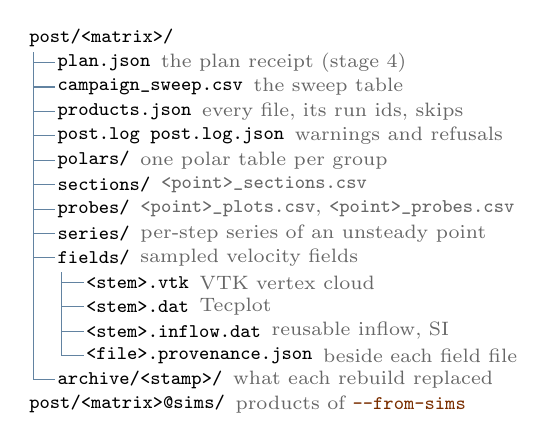
\begin{tikzpicture}
\tn{0}{0}{post/<matrix>/}{}
\tn{1}{1}{plan.json}{the plan receipt (stage 4)}
\tn{1}{2}{campaign_sweep.csv}{the sweep table}
\tn{1}{3}{products.json}{every file, its run ids, skips}
\tn{1}{4}{post.log post.log.json}{warnings and refusals}
\tn{1}{5}{polars/}{one polar table per group}
\tn{1}{6}{sections/}{\pth{<point>_sections.csv}}
\tn{1}{7}{probes/}{\pth{<point>_plots.csv}, \pth{<point>_probes.csv}}
\tn{1}{8}{series/}{per-step series of an unsteady point}
\tn{1}{9}{fields/}{sampled velocity fields}
\tn{2}{10}{<stem>.vtk}{VTK vertex cloud}
\tn{2}{11}{<stem>.dat}{Tecplot}
\tn{2}{12}{<stem>.inflow.dat}{reusable inflow, SI}
\tn{2}{13}{<file>.provenance.json}{beside each field file}
\tn{1}{14}{archive/<stamp>/}{what each rebuild replaced}
\tn{0}{15}{post/<matrix>@sims/}{products of \fl{--from-sims}}
\tv{0}{1}{14}
\tv{1}{10}{13}
\end{tikzpicture}

\hd{Sampled fields and their provenance}
Positions are in REFERENCE coordinates and meters, velocity absolute in REFERENCE components and m/s, one file per unsteady STEP. The provenance names the original frame, its recorded motion, the STEP, the coordinate conversion, the source-file hash and the velocity evidence. The convention was measured on one 26.124 build; a field of another 26.124 build is written with one warning per point and, in its \file{products.json} entry, \texttt{velocity\_convention} with \texttt{proven} false. To reuse an inflow file, state \texttt{FREESTREAM\_UNITS:SI} on the row.

\columnbreak
\hd{Commands}
\begin{cmdblock}{pyfs-matrix post}{[matrix]}{Rebuild the post-processed products from the records, with no solver.}
\opt{--workspace DIR}{the campaign root (default: current folder).}
\opt{--sims IDS}{only these simulations' products, in place; the super files stay as the last whole post wrote them.}
\opt{--runs NAME}{read another manifest, e.g. one a rebuild wrote.}
\opt{--from-sims}{ignore \file{runs.json}: records assembled in memory from \file{sims/}, for runs made outside the package; products to \file{post/<matrix>@sims/}.}
\opt{--steps-per-revolution N}{with \fl{--from-sims}: for a \texttt{LAST\_REVS\_AVG} window.}
\opt{--additional-pproc}{first reopen the final \texttt{.fsm} of each recorded point whose row states \texttt{ADDITIONAL\_PPROC}, with no solve, and extract that pproc; one solver launch per point; 26.124 only.}
\opt{--fs-version V}{\fl{--fs-exe PATH}, \fl{--local}, \fl{--recipe CODE=MODULE:FUNCTION}: for the additional post, as in run.}
\opt{--diagnostics}{print the recorded post diagnostics as Markdown, change nothing.}
\opt{--strict}{exit 3 when a product was skipped by design, after writing everything.}
\opt{--check-frozen}{refuse instead of warn (stage 6).}
\opt{--force-overwrite}{DESTROY products instead of archiving; asks first, and \fl{--yes} answers.}
\opt{--pproc-warnings}{grouped post-processing warnings; \fl{--verbose} every one in full.}
\end{cmdblock}

\hd{What the tables hold}
Every table opens with \texttt{POL}. A polar table has one row per point: the reference block, \texttt{J}, and the body, stability and wind axis coefficients. The probe table opens with \texttt{PROBE, X, Y, Z, FRAME, STEP}; a cell the package cannot fill reads \texttt{NA}, never blank.

\columnbreak
\hd{Files}
\rd{runs.json}{the records the products derive from.}
\rd{sims/sim_<POL>/datapoints/DP-<point>/}{each point's collected exports.}
\rd{sims/sim_<POL>/profiles/<POL>_probe_points.csv}{where each probe was, recorded at emission.}
\wf{post/<matrix>/}{the products, \file{products.json}, \file{post.log}, \file{post.log.json}.}
\wf{post/<matrix>/archive/<stamp>/}{what the rebuild replaced, one folder per rebuild.}
\wf{additional.json}{the record of the additional post; its files go to \file{datapoints/DP-<point>/additional/<pid>/}.}

\hd{Common errors}
\err{\fl{--yes} without \fl{--force-overwrite}.}{refused: it answers a question only that option asks.}
\err{A product is skipped by design (a polar under sideslip).}{named on standard error and under \texttt{skipped} in \file{products.json}; \fl{--diagnostics} prints why. Exit 0, or 3 with \fl{--strict}.}
\err{A field of another solver version, unit or export family.}{refused: \textit{native velocity convention has no evidence for this export/build/unit}. Measure the convention on that build first.}
\err{The matrix is in both homes with different bytes.}{the post warns naming both and builds from the run records; keep one copy.}
\err{The additional post on a workspace that submits from here.}{refused without \fl{--local}: only the local half is built.}
\err{A point's \texttt{.fsm} does not hash as its record says.}{skipped by name: the additional post reads only the file the run saved.}
\err{An old product is gone after a rebuild.}{it is in \file{post/<matrix>/archive/<stamp>/}; \cmd{pyfs-matrix restore} \texttt{products} brings back \file{products.json}.}

\hd{Where to read more}
Guide 5 and the page \textit{Post-processing definitions}, the definition of record of every product; the pages \textit{Sampled fields} and \textit{Extracting more from a finished point}.
\foot
\end{multicols}

% =====================================================================
\stagepage{8}{Maintenance: space, records and saved geometries}{A workspace grows and records go wrong. These commands measure and free space, delete simulations, mark a run failed after the fact, restore or rebuild the records, and clean a saved geometry. Each previews until \texttt{--apply}.}
\begin{multicols}{3}
\hd{What it is for}
Run the preview, read it, then apply. Every storage call, the preview included, is recorded in \file{storage_management.json}, and every rewrite of \file{runs.json} archives the previous copy first, so \cmd{pyfs-matrix restore} can undo it.

\hd{Figure: preview, apply, undo}
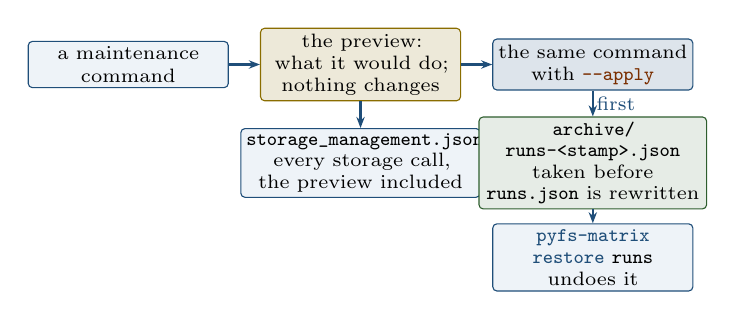
\begin{tikzpicture}
\node[box,text width=2.4cm] (cmd) at (0,0) {a maintenance command};
\node[box,text width=2.4cm,fill=wait!15,draw=wait] (pre) at (2.95,0) {the preview: what it would do; nothing changes};
\node[box,text width=2.4cm,fill=acc!15] (app) at (5.9,0) {the same command with \fl{--apply}};
\node[box,text width=2.9cm,font=\fontsize{6.6}{7.6}\selectfont] (log) at (2.95,-1.25) {\pth{storage_management.json}\\every storage call, the preview included};
\node[box,text width=2.75cm,font=\fontsize{6.6}{7.6}\selectfont,fill=ok!12,draw=ok] (arc) at (5.9,-1.25) {\pth{archive/}\\\pth{runs-<stamp>.json}\\taken before \pth{runs.json} is rewritten};
\node[box,text width=2.4cm] (rest) at (5.9,-2.45) {\cmd{pyfs-matrix restore} \pth{runs} undoes it};
\draw[arr] (cmd) -- (pre);
\draw[arr] (pre) -- (app);
\draw[arr] (pre) -- (log);
\draw[arr] (app) -- node[note,right]{first} (arc);
\draw[arr] (arc) -- (rest);
\end{tikzpicture}

\vspace{3pt}
\textbf{A storage recipe}, \file{inputs/management/m<id>.toml}, runs its tables in this order:\par
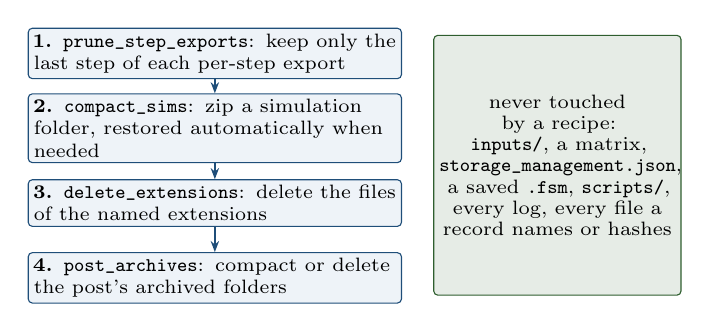
\begin{tikzpicture}
\node[box,text width=4.6cm,align=left] (n0) at (0,0) {\textbf{1.} \pth{prune_step_exports}: keep only the last step of each per-step export};
\node[box,text width=4.6cm,align=left] (n1) at (0,-0.95) {\textbf{2.} \pth{compact_sims}: zip a simulation folder, restored automatically when needed};
\node[box,text width=4.6cm,align=left] (n2) at (0,-1.9) {\textbf{3.} \pth{delete_extensions}: delete the files of the named extensions};
\node[box,text width=4.6cm,align=left] (n3) at (0,-2.85) {\textbf{4.} \pth{post_archives}: compact or delete the post's archived folders};
\draw[arr] (n0) -- (n1); \draw[arr] (n1) -- (n2); \draw[arr] (n2) -- (n3);
\node[box,text width=3.0cm,minimum height=3.3cm,fill=ok!12,draw=ok,font=\fontsize{6.6}{7.6}\selectfont] at (4.35,-1.42) {never touched by a recipe: \pth{inputs/}, a matrix, \pth{storage_management.json}, a saved \pth{.fsm}, \pth{scripts/}, every log, every file a record names or hashes};
\end{tikzpicture}

\begin{cmdblock}{pyfs-matrix inventory}{<geometry>}{Clean a saved simulation that keeps a previous run's unsteady solver actions.}
\opt{--clean}{remove them, keeping \file{<file>.bak-<stamp>}; a 26.120 file in meters is also reset to a fresh import, meshes and boundary conditions kept.}
\opt{--overwrite}{also rewrite the existing sidecar.}
\end{cmdblock}

\columnbreak
\hd{Commands}
\begin{cmdblock}{pyfs-matrix space-in-use}{}{Sizes on disk by top folder, by \file{sims/sim_*}, by extension; changes nothing.}
\opt{--top N}{rows per grouping (default 15). \fl{--workspace DIR}.}
\end{cmdblock}
\begin{cmdblock}{pyfs-matrix free-space}{<m-id>}{Run the recipe \file{inputs/management/m<id>.toml}.}
\opt{--apply}{change files (default: preview).}
\opt{--list}{every path each step touches, its size and what happens to it.}
\opt{--runs NAME}{also read this manifest; \fl{--workspace DIR}.}
\end{cmdblock}
\begin{cmdblock}{pyfs-matrix delete-sims}{<ids>}{Delete simulations (\texttt{4001,2009}), their products and records; a note row keeps the ids retired.}
\opt{--apply}{change files (default: preview).}
\opt{--force}{also a simulation whose run is still SUBMITTED.}
\opt{--matrix-products \{points-only,regenerate\}}{a product that also holds other points: leave it, marked stale, or post it again without the deleted ones.}
\opt{--runs NAME}{read and edit another manifest; \fl{--workspace DIR}.}
\end{cmdblock}
\begin{cmdblock}{pyfs-matrix mark-failed}{}{Every record of the named simulations becomes FAILED\_MARKED, its old status kept under \texttt{marked}.}
\opt{--sims IDS}{required: \texttt{2006,2007}.}
\opt{--reason TEXT}{why, recorded as given.}
\opt{--apply}{write (default: preview); \fl{--workspace DIR}.}
\end{cmdblock}
\begin{cmdblock}{pyfs-matrix restore}{{runs|storage|products|plan|additional}}{Bring a records file back from the archive, byte for byte.}
\opt{--apply}{write (default: preview); the current file is archived first.}
\opt{--stamp STAMP}{the copy to restore (default: the newest).}
\opt{--matrix STEM}{for products and plan, when several matrices have archives; \fl{--workspace DIR}.}
\end{cmdblock}
\begin{cmdblock}{pyfs-matrix rebuild}{}{Make run records again from \file{sims/}: each matrix row is rendered again and compared with the script that ran.}
\opt{--apply}{append the rebuilt records to \file{runs.json} (default: preview).}
\opt{--out NAME}{write them to another manifest instead, to compare.}
\opt{--all-sims}{every simulation folder, recorded or not; needs \fl{--out}.}
\opt{--sims IDS}{only these: \texttt{4001,2009}.}
\opt{--matrix FILE}{the matrix the simulations ran from.}
\opt{--build-alias BUILD=ALIAS}{the scheduler's name of a build then (repeatable).}
\opt{--inputs-from FOLDER}{another origin's \file{inputs/} for inputs changed after the run; \fl{--workspace DIR}.}
\end{cmdblock}
\begin{cmdblock}{pyfs-workspace archive}{<root> <sim_id>}{Zip one recorded simulation under \file{archive/} and remove its folder.}
\end{cmdblock}

\columnbreak
\hd{Files}
\rd{inputs/management/m<id>.toml}{the storage recipe.}
\wf{storage_management.json}{every storage call, \texttt{force} and the statuses included.}
\wf{runs.json}{rewritten by \cmd{pyfs-matrix delete-sims}, \cmd{pyfs-matrix mark-failed}, \cmd{pyfs-matrix rebuild}, \cmd{pyfs-matrix restore}.}
\wf{archive/runs-<stamp>.json}{the copy taken before each rewrite.}
\wf{sims/sim_<POL>.zip}{a simulation compacted by \texttt{compact\_sims}, restored automatically when needed.}
\wf{<file>.bak-<stamp>}{the geometry before \fl{--clean}.}

\hd{Common errors}
\err{\textit{have a run still SUBMITTED; collect it first}.}{run \cmd{pyfs-matrix collect}, or delete it anyway with \fl{--force}.}
\err{\fl{--apply} refuses, naming a product shared with other simulations.}{choose \fl{--matrix-products} \texttt{points-only} or \texttt{regenerate}; \texttt{regenerate} is refused with \fl{--runs}.}
\err{A simulation id with no record (mark-failed).}{refused by name before anything is written; a record already FAILED\_MARKED is left as it is.}
\err{The rebuild refuses an edited or drifted script, naming the input.}{the inputs changed after the run: \fl{--inputs-from} the folder they came from.}
\err{The profile no longer maps an old build.}{\fl{--build-alias} \texttt{26.123=26.12}.}
\err{A POL no current matrix holds.}{\fl{--matrix} the file the simulations ran from.}
\err{\fl{--out} names \file{runs.json} or a file that exists.}{refused before any work: choose a new name.}
\err{The restore is refused while \file{runs.json.lock} exists.}{a run, collect or sync is writing: wait for it.}
\err{A cleaned geometry has a new hash.}{runs staged before the clean keep theirs; a new campaign records the new one.}
\foot
\end{multicols}

\end{document}
